% This work is made available under the terms of the
% Creative Commons Attribution-ShareAlike 3.0 license, 
% http://creativecommons.org/licenses/by-sa/3.0/. 
%
% Version: $Revision$

\documentclass[a4paper]{book}

\usepackage{wrapfig}
\usepackage{graphicx}
\usepackage{hyperref}
\usepackage{multirow}
\usepackage{scalefnt}
\usepackage{tikz}

% watermark -- for draft stage
\usepackage[firstpage]{draftwatermark}
\SetWatermarkLightness{0.9}
\SetWatermarkScale{5}

% Copyright (c) 2009 by the University of Waikato, Hamilton, NZ. 
% This work is made available under the terms of the 
% Creative Commons Attribution-ShareAlike 3.0 license, 
% http://creativecommons.org/licenses/by-sa/3.0/. 
%
% Version: $Revision$

\newenvironment{tight_itemize}{
\begin{itemize}
  \setlength{\itemsep}{1pt}
  \setlength{\parskip}{0pt}
  \setlength{\parsep}{0pt}}{\end{itemize}
}

\newenvironment{tight_enumerate}{
\begin{enumerate}
  \setlength{\itemsep}{1pt}
  \setlength{\parskip}{0pt}
  \setlength{\parsep}{0pt}}{\end{enumerate}
}

% if you just need a simple heading
% Usage:
%   \heading{the text of the heading}
\newcommand{\heading}[1]{
  \vspace{0.3cm} \noindent \textbf{#1} \newline
}

\newcommand{\icon}[1]{\tikz[baseline=-3pt]\node[inner sep=0pt,outer sep=0pt]{\includegraphics[height=1.1em]{#1}};}


\title{
  \textbf{ADAMS} \\
  {\Large \textbf{A}dvanced \textbf{D}ata mining \textbf{A}nd \textbf{M}achine
  learning \textbf{S}ystem} \\
  {\Large Module: adams-weka} \\
  \vspace{1cm}
  
\includegraphics[width=2cm]{images/weka-module.png} \\
}
\author{
  Peter Reutemann
}

\setcounter{secnumdepth}{3}
\setcounter{tocdepth}{3}

\begin{document}

\begin{titlepage}
\maketitle

\thispagestyle{empty}
\center
\begin{table}[b]
	\begin{tabular}{c l l}
		\parbox[c][2cm]{2cm}{\copyright 2009-2016} &
		\parbox[c][2cm]{5cm}{
\includegraphics[width=5cm]{images/coat_of_arms.pdf}} \\
	\end{tabular}
	
\includegraphics[width=12cm]{images/cc.png} \\
\end{table}

\end{titlepage}

\tableofcontents
\listoffigures
%\listoftables

%%%%%%%%%%%%%%%%%%%%%%%%%%%%%%%%%%%
\chapter{Introduction}
The \textit{adams-weka} module offers most of the functionality found in WEKA
\cite{weka}: pre-processing, classification and regression, clustering,
attribute selection, data visualization and visualization of results/models.
But it does not stop there: the module also contains other features for
optimization, experiment generation that are not available from WEKA, be it
Explorer or KnowledgeFlow. It is assumed that you are familiar with
WEKA\footnote{If you haven't used WEKA before, check out the Data Mining book
\cite{wekabook}, which gives you a good introduction to machine learning, data
mining and WEKA.} and machine learning in general, as common terms are not
explained again.

If you have used WEKA's KnowledgeFlow before, then you will have to forget
(mostly) everything that you know about setting up workflows. ADAMS does things
quite differently in comparison to the WEKA. Additionally, ADAMS offers a range
of general purpose actors that allow you to go further.

The manual is split into several sections, with: \textit{classification and regression}
and \textit{clustering} comprising the most important sections.

% This work is made available under the terms of the
% Creative Commons Attribution-ShareAlike 4.0 license,
% http://creativecommons.org/licenses/by-sa/4.0/.
%
% Version: $Revision$

\chapter{Flow}
The \textit{adams-weka} module has a comprehensive set of actors and conversions
that allow you to build powerful flows using WEKA's functionality. The following
sections give a quick overview of available functionality. If you are interested
in flow examples, check out chapters \ref{classification_and_regression} and
\ref{clustering}.

\section{Conversions}
This module offers additional schemes for the \textit{Convert} transformer:
\begin{tight_itemize}
	\item \textit{AdamsInstanceToWekaInstance} -- converts an ADAMS instance
	into a WEKA one.
	\item \textit{MatchWekaInstanceAgainstFileHeader} -- uses a dataset header
	stored in a file to convert the string attributes of the instance passing 
	through into nominal ones (and vice versa).
	\item \textit{MatchWekaInstanceAgainstStorageHeader} -- uses a dataset
	header obtained from storage to convert the string attributes of the 
	instance passing through into nominal ones (and vice versa).
	\item \textit{ReportToWekaInstance} -- turns a \textit{Report} object
	into a WEKA instance.
	\item \textit{SpreadSheetToWekaInstances} -- turns a spreadsheet object
	into a WEKA dataset.
	\item \textit{WekaCapabilitiesToInstances} -- generates a dataset with
	random data that adheres to the capabilities retrieved from a
	\texttt{CapabilitiesHandler}.
	\item \textit{WekaDrawableString} -- exports the graph from a decision
	tree or bayesian network in 'dot' notation.
	\item \textit{WekaEvaluationToCostCurve} -- turns an Evaluation into
	cost curve data.
	\item \textit{WekaEvaluationToMaringCurve} -- turns an Evaluation into
	margin curve data.
	\item \textit{WekaEvaluationToThresholdCurve} -- turns an Evaluation into
	threshold curve data (eg ROC).
	\item \textit{WekaCapabilitiesToSpreadSheet} -- generates a spreadsheet
	with the  capabilities retrieved from a \texttt{CapabilitiesHandler}.
	\item \textit{WekaCommandToCode} -- turns a WEKA command-line into
	code snippets.
	\item \textit{WekaInstancesToSpreadSheet} -- turns a WEKA dataset into
	a spreadsheet object.
	\item \textit{WekaInstanceToAdamsInstance} -- turns a WEKA instance into
	an ADAMS one.
	\item \textit{WekaPredictionContainerToSpreadSheet} -- generates a 
	spreadsheet object from a prediction container (useful for display).
\end{tight_itemize}

\section{Conditions}
The following boolean conditions, e.g., used in the \textit{IfThenElse} or
\textit{Switch} control actors, are available:
\begin{tight_itemize}
	\item \textit{AdamsInstanceCapabilities} -- checks an ADAMS intance against
	the specified capabilities that it must satisfy.
	\item \textit{WekaCapabilities} -- checks a WEKA instance against the
	specified capabilities.
	\item \textit{WekaClassification} (used in conjunction with 
	\textit{Switch}) -- uses the returned classification index to determine 
	which branch of the switch statement should be used; for all other control 
	actors, the condition evaluates to ``true'' if an index is returnedl; 
	condition works only with nominal classes.
\end{tight_itemize}

\section{Actors}
The following sources are available:
\begin{tight_itemize}
	\item \textit{WekaClassifierGenerator} -- generates parameter sweeps for
	\item \textit{WekaClassifierSetup} -- outputs a single classifier setup.
	\item \textit{WekaClustererGenerator} -- generates parameter sweeps for
	\item \textit{WekaClustererSetup} -- outputs a single clusterer setup.
	\item \textit{WekaDatabaseReader} -- reads data from a database into
	WEKA's internal format.
	\item \textit{WekaDataGenerator} -- generates artificial data using WEKA's
	data generators.
	\item \textit{WekaFilterGenerator} -- generates parameter sweeps for
	filters.
	\item \textit{WekaNewExperiment} -- creates a new ADAMS experiment setup.
	\item \textit{WekaNewInstances} -- for generating empty datasets.
	\item \textit{WekaSelectDataset} -- for selecting datasets interactively.
	\item \textit{WekaSelectObjects} -- for selecting Weka objects, like
	classifiers.
\end{tight_itemize}
These transformers:
\begin{tight_itemize}
	\item \textit{WekaAccumulatedError} -- extracts all the errors
	collected during an evaluation, sorted according to magnitude and
	creates plot output, for comparing classifier performances (most useful
	for numeric classes).
	\item \textit{WekaAggregatedEvaluations} -- aggregates incoming
	Evaluation objects and forwards the current, aggregate state. 
	\item \textit{WekaAttributeIterator} -- iterates through the names of a
	dataset and outputs them.
	\item \textit{WekaAttributeSelection} -- for performing attribute selection.
	\item \textit{WekaAttributeSelectionSummary} -- generates a summary of the
	incoming attribute selection data.
	\item \textit{WekaCatSwarmOptimization} -- uses cat swarm optimization
	for parameter optimization.
	\item \textit{WekaChooseAttributes} -- allows the user to interactively
	select attributes to keep in a dataset.
	\item \textit{WekaClassifierInfo} -- outputs basic information about
	a classifier.
	\item \textit{WekaClassifierOptimizer} -- applies a classifier optimizer
	(e.g., GridSearch or MultiSearch) to a dataset and then forwards the best
	(untrained) setup.
	\item \textit{WekaClassifierRanker} -- evaluates an array of classifier
	setups on a dataset and outputs the top X performing setups.
	\item \textit{WekaClassifying} -- uses a serialized (or callable) model to
	make predictions on incoming data.
	\item \textit{WekaClassSelector} -- sets the class attribute in a dataset.
	\item \textit{WekaClusterAssignments} -- outputs the cluster assignments
	from a cluster evaluation.
	\item \textit{WekaClustererInfo} -- outputs basic info about a clusterer.
	\item \textit{WekaClusterEvaluationSummary} -- generates a summary string
	from a cluster evaluation object.
	\item \textit{WekaClustering} -- applies a serialized (or callable) model
	to incoming data.
	\item \textit{WekaCrossValidationClustererEvaluator} -- performs cross-validation
	on an incoming dataset using the referenced clusterer setup.
	\item \textit{WekaCrossValidationEvaluator} -- performs cross-validation
	on an incoming dataset using the referenced classifier setup.
	\item \textit{WekaCrossValidationSplit} -- generates train/test set splits
	like cross-validation would generate.
	\item \textit{WekaEvaluationInfo} -- outputs basic info about a Weka
	Evaluation object.
	\item \textit{WekaEvaluationPostProcessor} -- allows post-processing
	of Evaluation objects, e.g., extraction sub-ranges.
	\item \textit{WekaEvaluationSummary} -- generates a summary for an
	Evaluation.
	\item \textit{WekaEvaluationValuePicker} -- retrieves a single statistic
	from an Evaluation.
	\item \textit{WekaEvaluationValues} -- generates a spreadsheet with the
	selected statistics from an Evaluation.
	\item \textit{WekaExperiment} -- executes a WEKA experiment, like in the 
	Experimenter.
	\item \textit{WekaExperimentEvaluation} -- evaluates a WEKA experiment,
	generating text output of various sorts.
	\item \textit{WekaExperimentExecution} -- executes an incoming ADAMS
	experiment.
	\item \textit{WekaExperimentFileReader} -- reads an experiment from disk.
	\item \textit{WekaExtractArray} -- extracts a row or column from a WEKA
	dataset (using the internal format).
	\item \textit{WekaExtractPLSMatrix} -- extracts PLS matrices from in
	incoming PLS classifier (or scheme that gives access to internal PLS matrices).
	\item \textit{WekaFileReader} -- reads any dataset that WEKA can handle,
	either outputs the header, the complete dataset or row-by-row.
	\item \textit{WekaFilter} -- applies a WEKA filter to the data.
	\item \textit{WekaGenericPLSMatrixAccess} -- extracts PLS matrices from in
	incoming PLS classifier (or scheme that gives access to internal PLS matrices).
	\item \textit{WekaGeneticAlgorithm} -- applies the specified genetic
	algorithm to the incoming dataset, e.g., for parameter optimization.
	\item \textit{WekaGetCapabilities} -- retrieves the capabilities of a
	\texttt{CapabilitiesHandler} (e.g., Filter or Classifier).
	\item \textit{WekaGetInstanceValue} -- retrieves an attribute's value from
	a dataset row.
	\item \textit{WekaGetInstancesValue} -- retrieves an attribute's value from
	a dataset.
	\item \textit{WekaInstanceBuffer} -- buffers either incoming instance 
	objects and outputs datasets or outputs instance objects when getting
	datasets.
	\item \textit{WekaInstanceDumper} -- for dumping dataset rows into files,
	one row at a time (ARFF or CSV).
	\item \textit{WekaInstanceEvaluator} -- adds an attribute with the value
	returned by an instance evaluator.
	\item \textit{WekaInstanceFileReader} -- outputs ADAMS instance objects.
	\item \textit{WekaInstancesAppend} -- creates one large dataset from 
	multiple ones, by appending them one after the other.
	\item \textit{WekaInstancesInfo} -- outputs information on a dataset.
	\item \textit{WekaInstancesMerge} -- allows the merging of several datasets 
	(side-by-side).
	\item \textit{WekaInstancesStatistic} -- computes statistics on rows
	or columns of an Instances object.
	\item \textit{WekaInstanceStreamPlotGenerator} -- generates plot containers
	from a range of attributes of instance objects passing through (i.e., you 
	can plot several attributes in one go).
	\item \textit{WekaModelReader} -- reads a serialized model.
	\item \textit{WekaMultiLabelSplitter} -- splits a datasets with multiple
	class attributes (``multi-label'') into ones with only a single class 
	attribute.
	\item \textit{WekaNewInstance} -- creates an instance object with only 
	missing values using a dataset as template.
	\item \textit{WekaPredictionsToInstances} -- turns WEKA predictions into
	a WEKA dataset (actual, predicted, etc).
	\item \textit{WekaPredictionsToSpreadSheet} -- turns WEKA predictions into
	a spreadsheet (actual, predicted, etc).
	\item \textit{WekaPrincipalComponents} -- outputs loadings and transformed
	data obtained from principal components analysis.
	\item \textit{WekaRandomSplit} -- generates a random split of a dataset.
	\item \textit{WekaRegexToRange} -- generates a range string using a regular
	expression applied to the names of a dataset.
	\item \textit{WekaRenameRelation} -- renames a dataset.
	\item \textit{WekaReorderAttributesToReference} -- reorders the attributes
	in incoming Instance/Instances based on an order defined in a reference
	dataset (callable actor or file).
	\item \textit{WekaSetInstanceValue} -- sets a specific attribute value in
	an instance object.
	\item \textit{WekaSetInstancesValue} -- sets a specific attribute value in
	a dataset object.
	\item \textit{WekaSpreadSheetToPredictions} -- turns a spreadsheet back
	into a fake Evaluation object. Allows processing of actual/predicted data
	from other applications.
	\item \textit{WekaStoreInstance} -- appends the passing through instance
	\item \textit{WekaStreamEvaluator} -- performs prequential evaluation
	of an incremental classifier on a data stream.
	\item \textit{WekaStreamFilter} -- works the same as
	\textit{WekaFilter} but only allows stream filters to be selected.
	\item \textit{WekaSubsets} -- splits dataset into subsets using the unique
	values of an attribute to identify subsets.
	\item \textit{WekaTestSetClustererEvaluator} -- evaluates a trained
	clusterer on a dataset obtained from a callable actor.
	\item \textit{WekaTestSetEvaluator} -- evaluates a trained classifier on
	a dataset obtained from a callable actor.
	\item \textit{WekaTextDiectoryReader} -- reads in a directory with the 
	documents in the sub-directories representing different classes.
	\item \textit{WekaTrainClassifier} -- used for generating a trained
	model using a dataset.
	\item \textit{WekaTrainClusterer} -- trains a cluster algorithm setup
	on a dataset.
	\item \textit{WekaTrainTestSetClustererEvaluator} -- evaluates a referenced
	clusterer using the incoming train/test split.
	\item \textit{WekaTrainTestSetEvaluator} -- evaluates a referenced classifier
	using the incoming train/test split.
\end{tight_itemize}
And these sinks:
\begin{tight_itemize}
	\item \textit{WekaAttributeSummary} -- displays the summary of one or more attributes.
	\item \textit{WekaClassifierErrors} -- displays the errors of a classifier.
	\item \textit{WekaCostBenefitAnalysis} -- displays a cost-benefit analysis dialog.
	\item \textit{WekaCostCurve} -- generates a cost curve.
	\item \textit{WekaDatabaseWriter} -- writes a dataset to a database.
	\item \textit{WekaExperimentFileWriter} -- writes an ADAMS experiment to disk.
	\item \textit{WekaExperimentGenerator} -- generates a WEKA experiment by
	adding the incoming classifier setups and writing it to disk.
	\item \textit{WekaFileWriter} -- writes a dataset to any file format that
	WEKA can handle.
	\item \textit{WekaGraphVisualizer} -- displays a Bayesian network (from XML or BIF).
	\item \textit{WekaInstancesDisplay} -- displays datasets in table format.
	\item \textit{WekaInstancesPlot} -- plots one attribute vs another.
	\item \textit{WekaInstanceViewer} -- visualizes incoming WEKA or ADAMS
	instance objects the same way as the \textit{Instance Explorer} tool does.
	\item \textit{WekaMarginCurve} -- displays a margin curve.
	\item \textit{WekaModelWriter} -- writes a model container or
	classifier/clusterer to disk.
	\item \textit{WekaThresholdCurve} -- displays threshold curves like, 
	receiver-operator curve (ROC) or precision/recall.
	\item \textit{WekaTreeVisualizer} -- displays a tree in 'dot' notation.
\end{tight_itemize}

\section{Templates}
Here are some templates that make the flow development for WEKA easier:
\begin{tight_itemize}
	\item \textit{InstanceDumperVariable} -- generates a variable for the 
	\textit{WekaInstanceDumper} actor which contains an ARFF/CSV filename 
	prefix aligned with the flow's filename, i.e., the ARFF/CSV file will 
	always get placed in the same location as the flow.
\end{tight_itemize}


% This work is made available under the terms of the
% Creative Commons Attribution-ShareAlike 4.0 license,
% http://creativecommons.org/licenses/by-sa/4.0/.

\chapter{Classification and Regression}
\label{classification_and_regression}
WEKA's main strength lies in its large number of classification and regression
schemes. Most of the documentation will cover this functionality therefore.

We start out with some basic WEKA functionality, like loading and
preprocessing data, building models and evaluating them. That includes
visualization of the results and models as well. After that we will cover more
advanced features like learning
curves, experiment generation/evaluation and optimization of classifiers in ADAMS.

\newpage
\section{Basic}
In this section we describe how to perform basic WEKA functionality that you are
used to perform with the Explorer, but in the workflow context. Instead of
having to repeat the same steps, like loading and preprocessing data, whenever
you update your data, a flow allows you to define the steps apriori and then merely
re-execute them time and time again. Also, flows make it very easy to
\textit{document} all the steps that you perform, not just merely recording what
you are doing.

\subsection{Loading data}
Before we can build any models, we have to have data at hand, of course. So the
first step will be to obtain data from somewhere, whether that is by loading a
local dataset or by downloading a remote dataset.

To start, we will be loading files that are stored locally. The actor used for
loading datasets is the \textit{WekaFileReader} transformer. This actor does not
have an option for the file to load. Instead, it expects a file name, string or
URL object to arrive at its input port. In order to supply a local file, we use
the \textit{SingleFileSupplier} source, which allows us to specify a single file
that gets forwarded in the flow. If required, one can also use the
\textit{MultiFileSupplier} or \textit{DirectoryLister}
sources\footnote{adams-weka-crossvalidate\_classifier\_multiple\_datasets.flow},
which can forward multiple file names instead of just one. The latter one is
especially handy, if the files are not known in advance, e.g., generated on the
fly. In order to display the loaded data, we use the
\textit{WekaInstancesDisplay} sink actor, which displays the data in a nice
tabular format. Figure \ref{basic-load_local_dataset} shows the flow for loading
the dataset and Figure \ref{basic-load_local_dataset-output} the generated
output.

\begin{figure}[ht]
  \begin{minipage}[t]{0.5\linewidth}
    \centering
    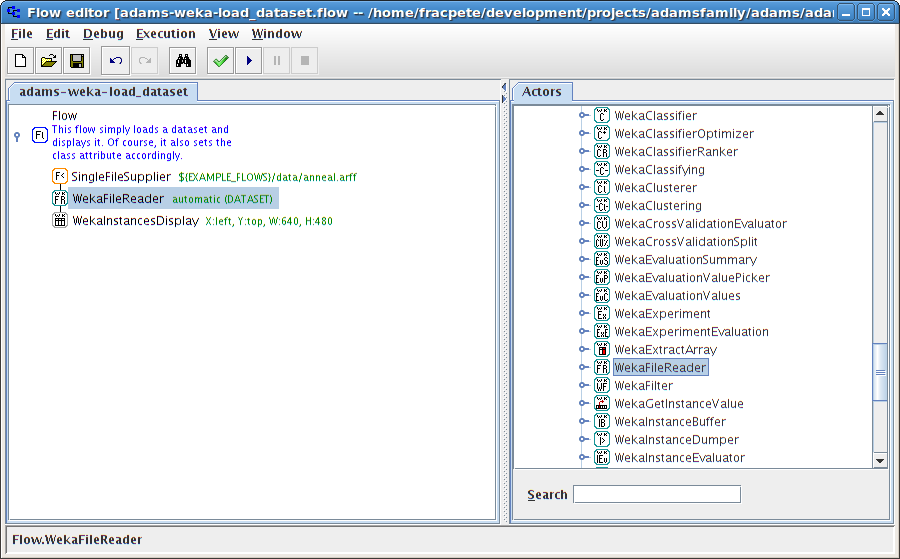
\includegraphics[width=6.0cm]{images/basic-load_local_dataset.png}
    \caption{Flow for loading a local dataset.}
    \label{basic-load_local_dataset}
  \end{minipage}
  \hspace{0.5cm}
  \begin{minipage}[t]{0.5\linewidth}
    \centering
    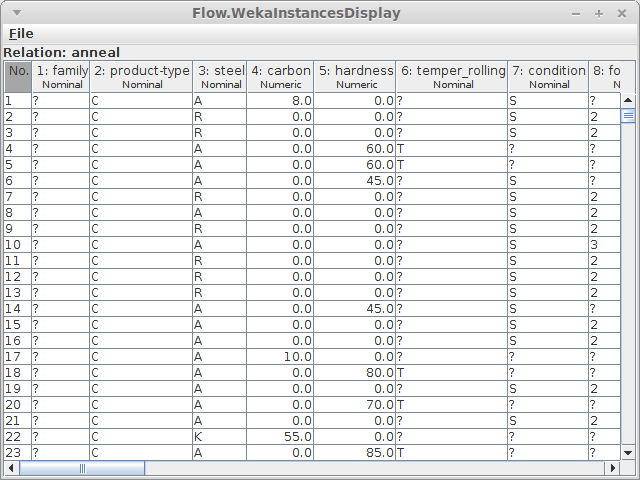
\includegraphics[width=5.0cm]{images/basic-load_local_dataset-output.png}
    \caption{The dataset that got loaded from disk.}
    \label{basic-load_local_dataset-output}
  \end{minipage}
\end{figure}

In this example\footnote{adams-weka-load\_dataset.flow} we let the
\textit{WekaFileReader} determine the correct file loader automatically, based
on the file extension. If this automatic determination should fail, you can
always check the ``useCustomLoader'' checkbox and then configure the appropriate
loader yourself.

Another feature of this actor is the ability to output the dataset row by row
(option ``incremental''). This is very handy in case of very large files, where
loading into memory could pose a problem. Even though the incremental feature
works for any file type that WEKA can read, truly incremental, i.e.,
memory-efficient, loading is only possible if the underlying loader also
supports incremental loading. In any other case, the dataset gets loaded fully
into memory before being forwarded row by row.

Finally, artificial data can be generated within ADAMS as well. Using the
\textit{WekaDataGenerator} source, any WEKA data generator can be used to output
data. The flow\footnote{adams-weka-data\_generator.flow} depicted in Figure
\ref{basic-datagenerator} generates a small dataset using the ``Agrawal'' data
generator.

\begin{figure}[htb]
  \centering
  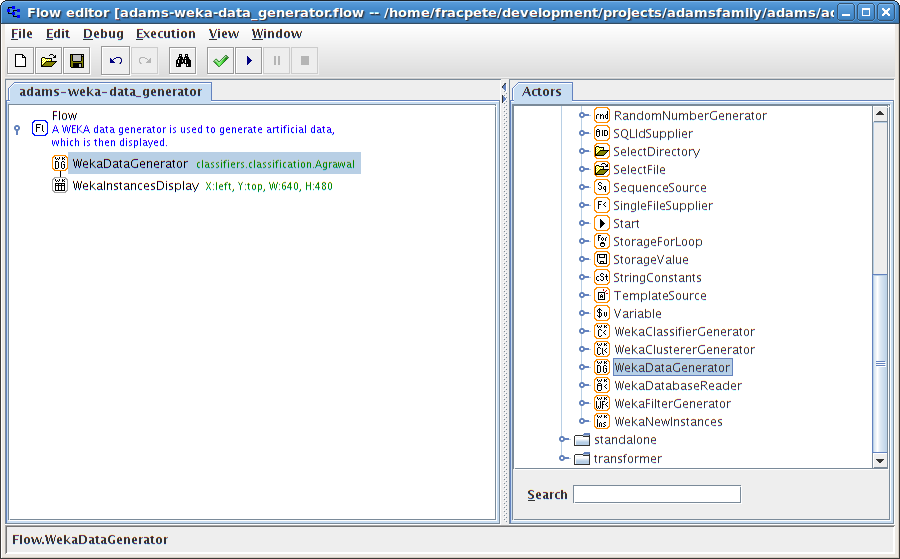
\includegraphics[width=6.0cm]{images/basic-datagenerator.png}
  \caption{Flow for generating and displaying an artificial dataset.}
  \label{basic-datagenerator}
\end{figure}

\subsection{Building models}
After having sorted out the loading of the data, it is time to check out how to
build models. Since we are using supervised algorithms, we have to make sure
that the datasets have a class attribute set. The \textit{WekaClassSelector}
actor allows the setting of the class attribute, in the default setting it
simply uses the last attribute as the class attribute. With the
\textit{WekaTrainClassifier} actor you can choose a callable classifier to be built. 
You define a callable classifier by adding a \textit{WekaClassifierSetup} source
to the \textit{CallableActors} standalone, which you then reference in your 
\textit{WekaTrainClassifier} actor.
By default, the \textit{WekaTrainClassifier} actor outputs a container that comprises
the built model and the header of the training set. In order to extract either
of the container items, you need to use the \textit{ContainerValuePicker}
control actor. Figure \ref{basic-building_model1-flow} demonstrates how to train
a J48 classifier on dataset and then displaying the built model (see Figure
\ref{basic-building_model1-output})\footnote{adams-weka-build\_classifier-output\_only\_model.flow}.

\begin{figure}[ht]
  \begin{minipage}[t]{0.5\linewidth}
    \centering
    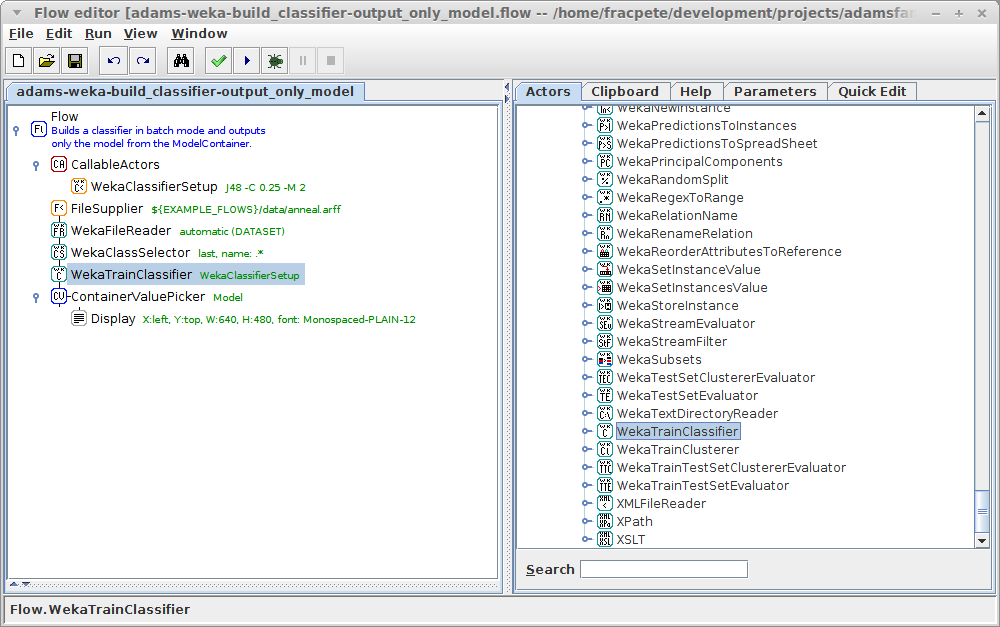
\includegraphics[width=6.0cm]{images/basic-building_model1-flow.png}
    \caption{Flow for building J48 model on a dataset and outputting the model.}
    \label{basic-building_model1-flow}
  \end{minipage}
  \hspace{0.5cm}
  \begin{minipage}[t]{0.5\linewidth}
    \centering
    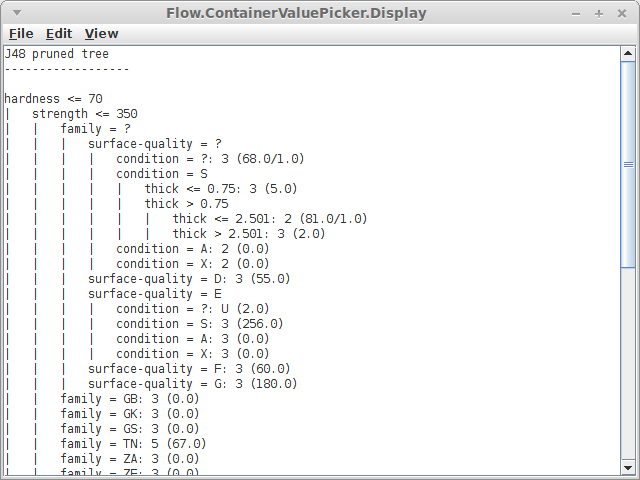
\includegraphics[width=5.5cm]{images/basic-building_model1-output.png}
    \caption{J48 model output.}
    \label{basic-building_model1-output}
  \end{minipage}
\end{figure}

A built model can be saved to disk (and then re-used later) using the
\textit{WekaModelWriter}. The file generated can also be loaded in the WEKA
Explorer again and applied to another test set
there\footnote{adams-weka-build\_classifier-save\_model.flow}.

\subsection{Preprocessing}
A very important, but often underrated step is preprocessing. Unless your data
is properly cleaned up and in the right format, your models will not be very
meaningful. Preprocessing steps can be done within the flow using the
\textit{WekaFilter} transformer, which wraps around a single WEKA filter. One
either chains multiple actors together or uses the
\textit{weka.filters.MultiFilter} meta-filter to executed several filter
sequentially in a single actor.

In Figure \ref{basic-preprocessing_flow} we are investigating the impact of
preprocessing on the ``slug'' dataset \cite{slug}. The
flow\footnote{adams-weka-filter\_data.flow} cross-validates
\textit{LinearRegression} on the original and log-transformed data. The
log-transformed data is generated by applying the \textit{AddExpression} filter
on each of the two attributes of the dataset and then deleting the original
ones. In each case, original or preprocessed, it displays the evaluation summary
and classifier errors.

\begin{figure}[htb]
  \centering
  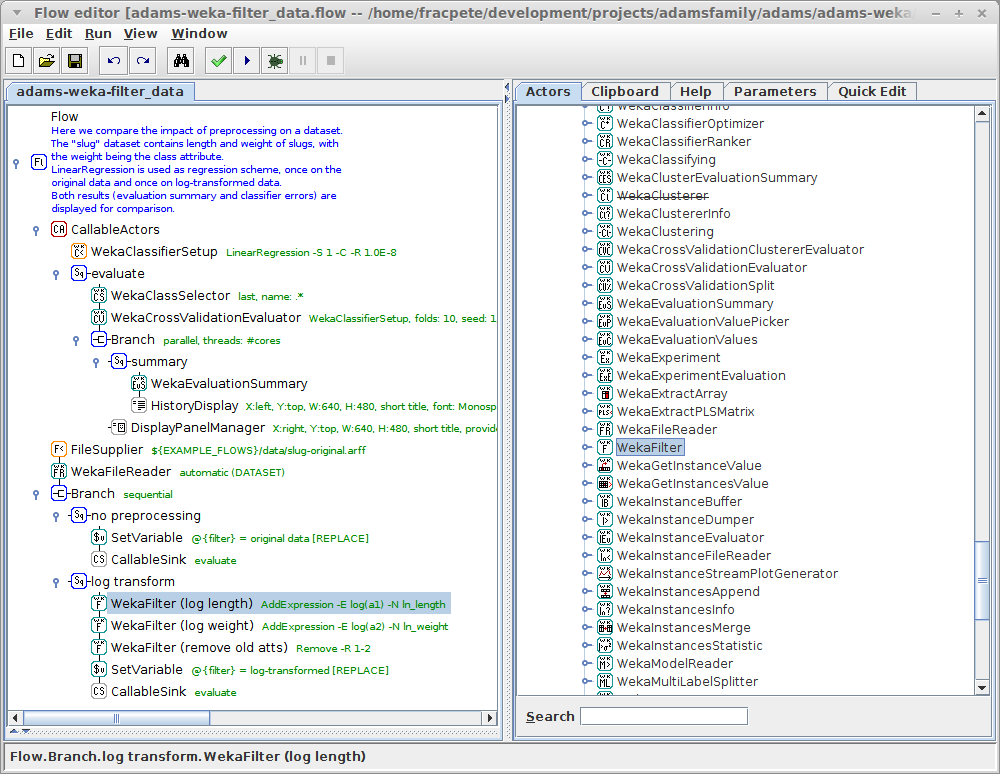
\includegraphics[width=7.0cm]{images/basic-preprocessing_flow.png}
  \caption{Flow for comparing results generated from original and preprocessed
  ``slug'' data \cite{slug}.}
  \label{basic-preprocessing_flow}
\end{figure}

Figures \ref{basic-preprocessing_summary-original} and
\ref{basic-preprocessing_summary-log} show the evaluation summary, for the
original and the log-transformed data. The log-transformed dataset gets not
only a better correlation coefficient, but also smaller errors.

\begin{figure}[ht]
  \begin{minipage}[t]{0.5\linewidth}
    \centering
    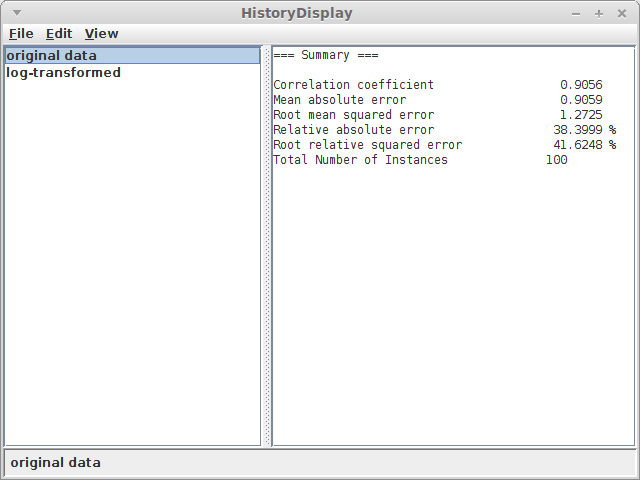
\includegraphics[width=5.5cm]{images/basic-preprocessing_summary-original.png}
    \caption{Evaluation summary on ``slug'' dataset (original).}
    \label{basic-preprocessing_summary-original}
  \end{minipage}
  \hspace{0.5cm}
  \begin{minipage}[t]{0.5\linewidth}
    \centering
    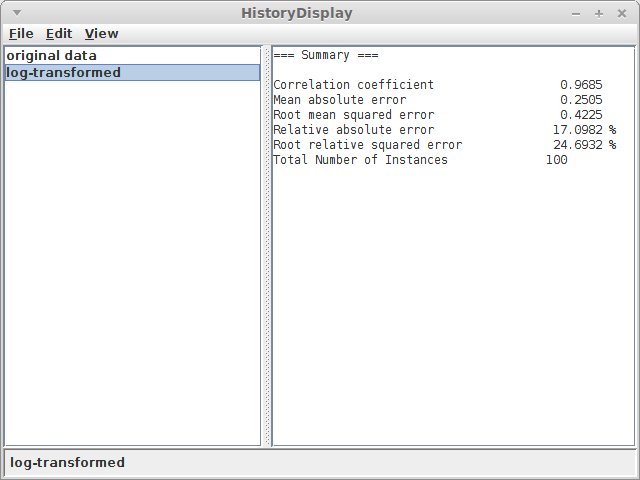
\includegraphics[width=5.5cm]{images/basic-preprocessing_summary-log.png}
    \caption{Evaluation summary on ``slug'' dataset (log-transformed).}
    \label{basic-preprocessing_summary-log}
  \end{minipage}
\end{figure}

Figures \ref{basic-preprocessing_errors-original} and
\ref{basic-preprocessing_errors-log} display the classifier errors. It is
obvious from the funy log-shaped curve, that LinearRegression built on the
original data is not a very good model. Something that is not so obvious by just
looking at the correlation coefficient: 0.9056 is not bad.

\begin{figure}[ht]
  \begin{minipage}[t]{0.5\linewidth}
    \centering
    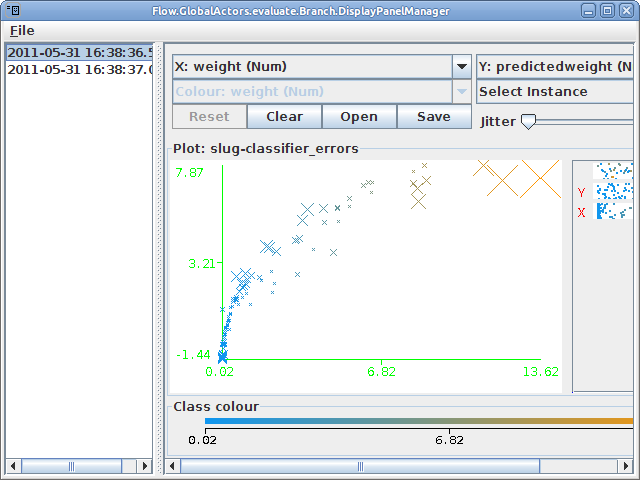
\includegraphics[width=5.5cm]{images/basic-preprocessing_errors-original.png}
    \caption{Classifier errors on ``slug'' dataset (original).}
    \label{basic-preprocessing_errors-original}
  \end{minipage}
  \hspace{0.5cm}
  \begin{minipage}[t]{0.5\linewidth}
    \centering
    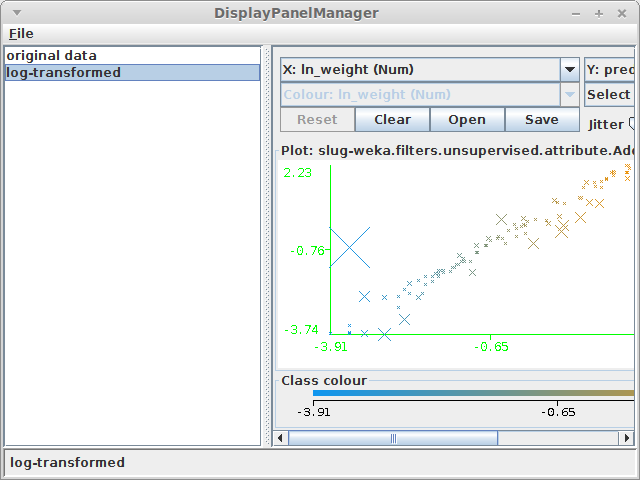
\includegraphics[width=5.5cm]{images/basic-preprocessing_errors-log.png}
    \caption{Classifier errors on ``slug'' dataset (log-transformed).}
    \label{basic-preprocessing_errors-log}
  \end{minipage}
\end{figure}

This flow can be quickly extended to accommodate other preprocessing techniques,
all very easily comparable in the graphical output.

In this example the preprocessing was rather specific. On the other hand, if
your are working mainly in a particular data domain, like spectral analysis of
some kind, then certain preprocessing steps will always be same. In this case,
it makes sense to store these externally in a \textit{preprocessing library}
which you then link to using external actors (see manual for the
\textit{adams-core} module for more details). This reduces duplication and you
will only have to update the preprocessing step in a single location.

Instead of batch-filtering data, you can also filter streams of 
\textit{weka.core.Instance} objects, using the \textit{WekaStreamFilter}
transformer. This filter offers a subset of WEKA's filters, which don't need
a batch of data to be initialized with before being able to process data.

\clearpage
\subsection{Evaluation}
Knowing how to build a model is good, but how can you tell whether the model
that you built is any good? Evaluation is the key to unlock this mystery.
ADAMS offers several types of evaluations:
\begin{tight_itemize}
	\item \textit{Cross-validation} -- if you only have a single dataset.
	\item \textit{Test set evaluation} -- evaluating an already trained classifier
	with a separate dataset.
	\item \textit{Train/test set evaluation} -- training and evaluating a
	classifier with a training and test set. This can be either achieved using a
	\textit{RandomSplit} actor or reading two separate files from disk.
\end{tight_itemize}

\heading{Cross-validation}
We start with cross-validation, which is probably the most used type of
evaluation. The \textit{WekaCrossValidationEvaluator} transformer is used for
cross-validation. In order to get around ADAMS' limitation of allowing only one
input, the \textit{WekaCrossValidationEvaluator} actor takes a dataset as input
and obtains the classifier to evaluate from a \textit{callable actor}. This
approach hides \textit{how} the classifier is obtained, whether it is a simple
\textit{WekaClassifierSetup} definition or a more complex scheme for outputting a
\textit{Classifier} object (e.g., loading it from a serialized model file).
Figure \ref{basic-crossvalidate1-flow} shows a
flow\footnote{adams-weka-crossvalidate\_classifier.flow} with simple
cross-validation using a callable \textit{WekaClassifierSetup} to obtain the classifier
object from.

\begin{figure}[ht]
  \begin{minipage}[t]{0.5\linewidth}
    \centering
    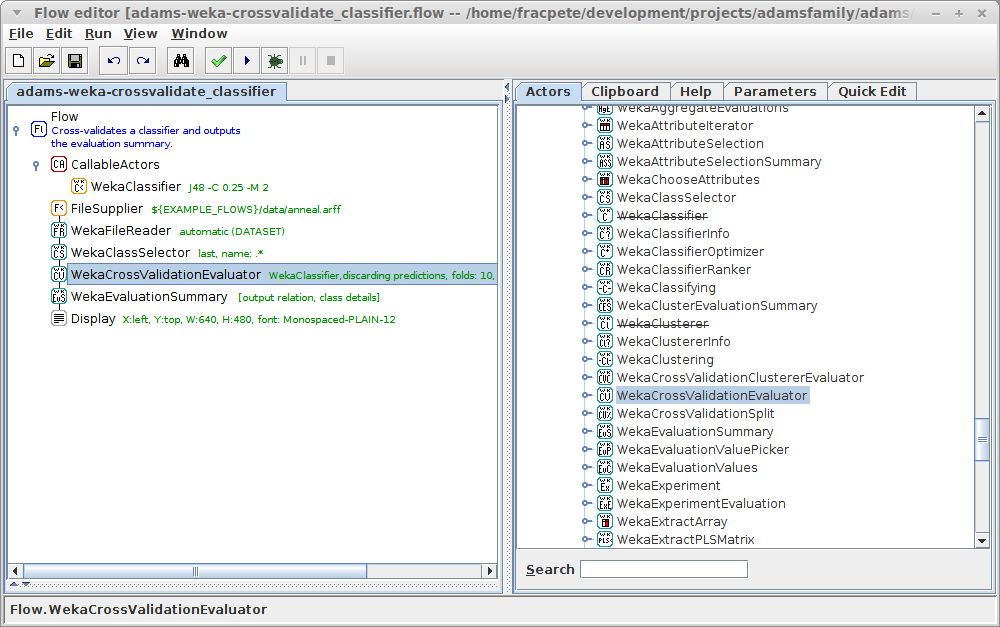
\includegraphics[width=6.0cm]{images/basic-crossvalidate1-flow.png}
    \caption{Cross-validating a classifier and outputting the summary.}
    \label{basic-crossvalidate1-flow}
  \end{minipage}
  \hspace{0.5cm}
  \begin{minipage}[t]{0.5\linewidth}
    \centering
    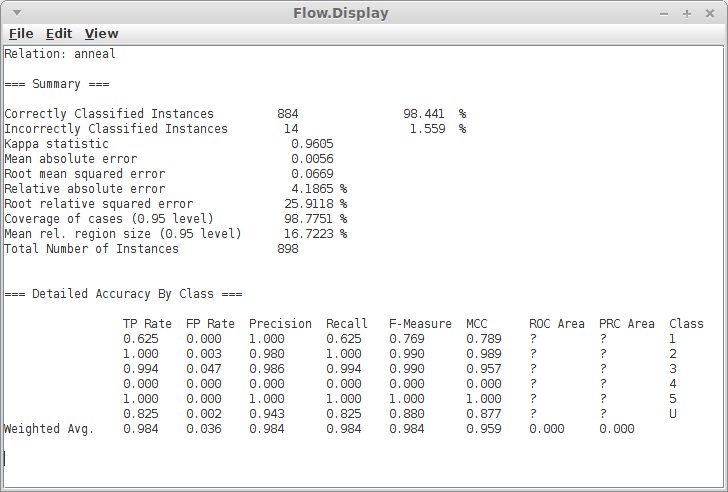
\includegraphics[width=5.5cm]{images/basic-crossvalidate1-output.png}
    \caption{Summary output of a cross-validated classifier.}
    \label{basic-crossvalidate1-output}
  \end{minipage}
\end{figure}

Most of the time, you don't just want to test a single classifier, but several
ones. With ADAMS you can, for instance, load classifier command-lines from a
text file and then evaluate them one after the
after\footnote{adams-weka-crossvalidate\_classifier\_setups\_from\_text\_file.flow}.
Reading the text file (see Figure
\ref{basic-crossvalidate_multiple_files-setups}) is fairly straight-forward,
using the \textit{TextFileReader} transformer.

\begin{figure}[htb]
  \centering
  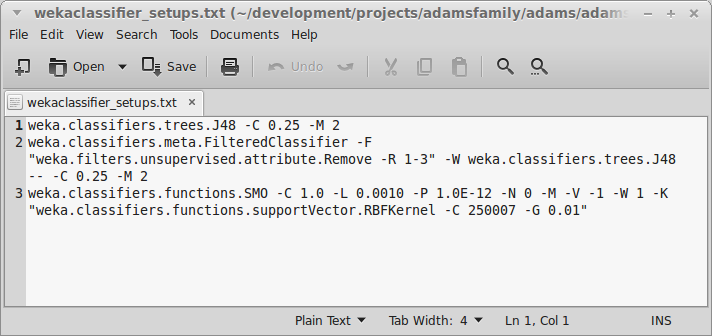
\includegraphics[width=6.0cm]{images/basic-crossvalidate_multiple_files-setups.png}
  \caption{Text file with command-lines of various classifiers.}
  \label{basic-crossvalidate_multiple_files-setups}
\end{figure}

For updating the callable classifier's set up, we need to attach a variable to the
callable \textit{WekaClassifierSetup} actor's ``classifier'' option and update this
variable with each set up that we are reading from the text file using the
\textit{SetVariable} transformer. This update of the classifier set up has to
happen before we are triggering the cross-validation. Figures
\ref{basic-crossvalidate_multiple_files-flow} and
\ref{basic-crossvalidate_multiple_files-output} show the full flow and the
generated output, when reading in three set ups from a text file (J48,
filtered J48, SMO).

\begin{figure}[ht]
  \begin{minipage}[t]{0.5\linewidth}
    \centering
    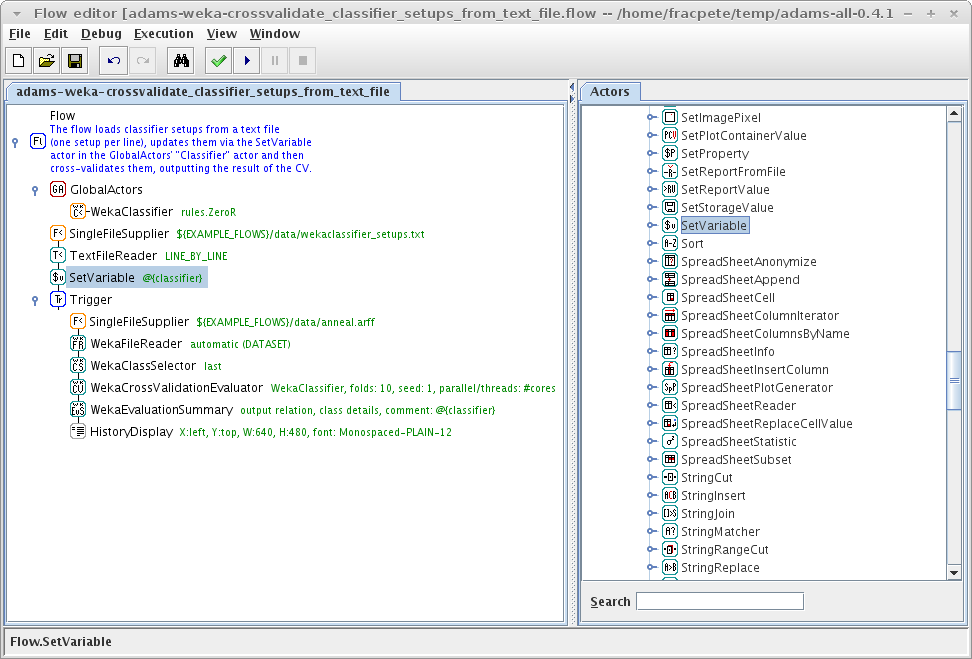
\includegraphics[width=6.0cm]{images/basic-crossvalidate_multiple_files-flow.png}
    \caption{Cross-validating classifier set ups read from a text file and
    displaying the evaluation summaries.}
    \label{basic-crossvalidate_multiple_files-flow}
  \end{minipage}
  \hspace{0.5cm}
  \begin{minipage}[t]{0.5\linewidth}
    \centering
    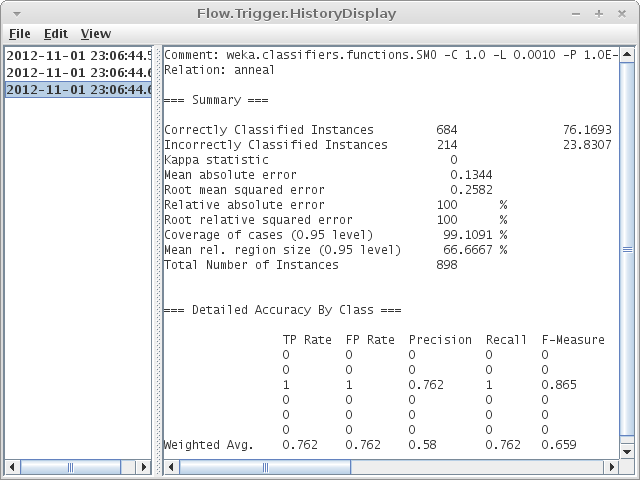
\includegraphics[width=5.5cm]{images/basic-crossvalidate_multiple_files-output.png}
    \caption{Summary outputs of cross-validated classifiers.}
    \label{basic-crossvalidate_multiple_files-output}
  \end{minipage}
\end{figure}

\heading{Test set evaluation}
Simply testing a built classifier on a test set is useful when you are always
intending to save the generated model to a file, but also want to keep an eye on
the performance. In this case, you can very easily extend your current flow for
building and saving the model. First, add a callable actor that loads the separate
training set from disk. Second, add a \textit{Tee} control actor that performs
the evaluation using the \textit{WekaTestSetEvaluator} and
\textit{WekaEvaluationSummary} transformers and a \textit{Display} sink for
showing the
results\footnote{adams-weka-build\_classifier\_evaluate\_on\_testset.flow}. The
full flow and the generated output are shown in Figures
\ref{basic-testseteval-flow} and \ref{basic-testseteval-output}.

\begin{figure}[ht]
  \begin{minipage}[t]{0.5\linewidth}
    \centering
    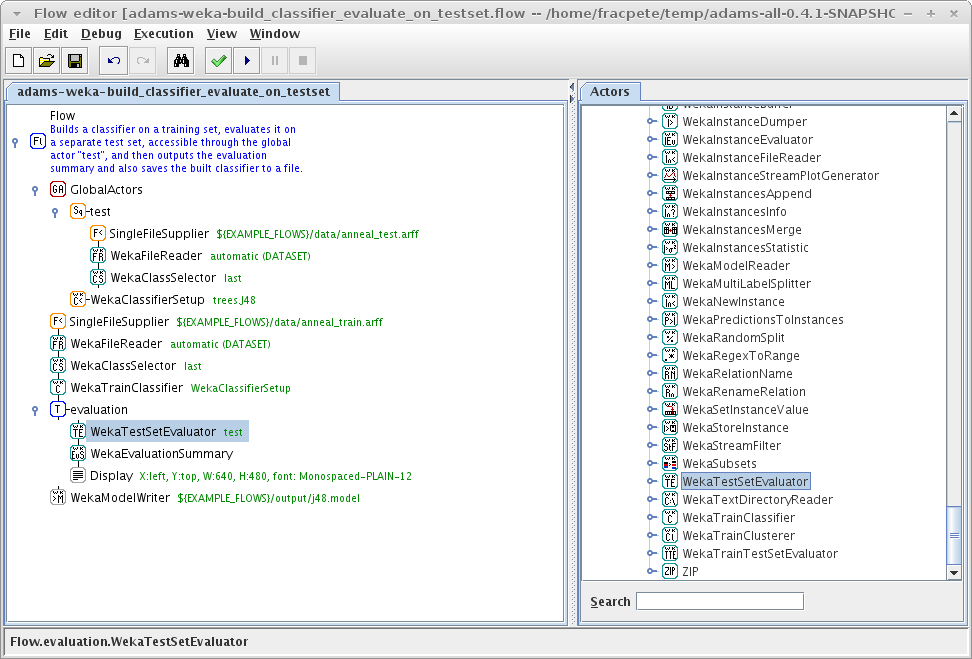
\includegraphics[width=6.0cm]{images/basic-testseteval-flow.png}
    \caption{Flow for evaluating built classifier on a separate test set.}
    \label{basic-testseteval-flow}
  \end{minipage}
  \hspace{0.5cm}
  \begin{minipage}[t]{0.5\linewidth}
    \centering
    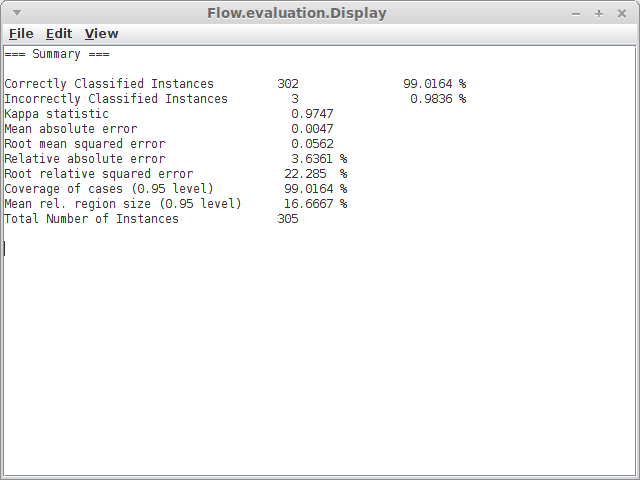
\includegraphics[width=5.5cm]{images/basic-testseteval-output.png}
    \caption{Summary output of classifier evaluated on separate test set.}
    \label{basic-testseteval-output}
  \end{minipage}
\end{figure}

\heading{Train/test set evaluation}
An evaluation using separate train and test set can be used, if you don't want
to keep the evaluated model, but you are only interested in the evaluation
output. The evaluation actor in this case is the
\textit{WekaTrainTestSetEvaluator} transformer. This actor accepts
\textit{WekaTrainTestSetContainer} data tokens. To generate this container you
have several options:
\begin{tight_itemize}
	\item \textit{WekaRandomSplit} -- splits a single dataset into a train and test
	set, based on the percentage supplied by the user.
	\item \textit{WekaCrossValidationSplit} -- Generates train/test splits like
	they occur in cross-validation. Useful, if you want to inspect the various models
	built during cross-validation, not just the summary.
	\item \textit{MakeContainer} -- manually generating a container from two
	individually loaded datasets.
\end{tight_itemize}

Figures \ref{basic-randomspliteval-flow} and \ref{basic-randomspliteval-output}
show how to use the \textit{RandomSplit} actor in the evaluation
process\footnote{adams-weka-evaluate\_classifier\_randomsplit.flow}. For
simulating cross-validation, simply exchange the \textit{WekaRandomSplit} actor
with a \textit{WekaCrossValidationSplit} one (you might also want to change from
\textit{Display} to \textit{HistoryDisplay}, to keep better track of the various
evaluations).

\begin{figure}[ht]
  \begin{minipage}[t]{0.5\linewidth}
    \centering
    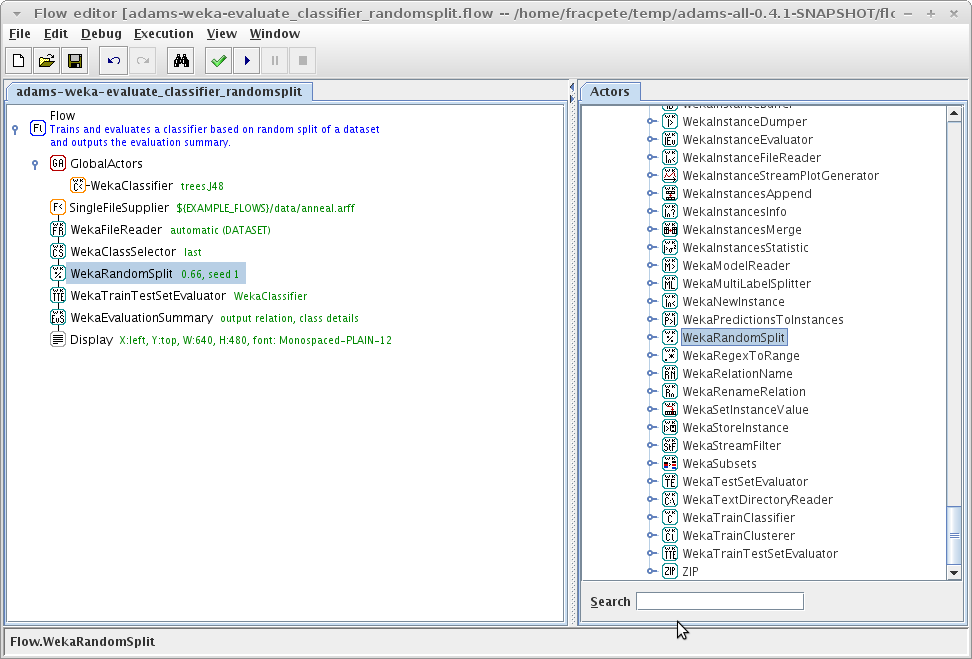
\includegraphics[width=6.0cm]{images/basic-randomspliteval-flow.png}
    \caption{Flow for building/evaluating classifier on a random split.}
    \label{basic-randomspliteval-flow}
  \end{minipage}
  \hspace{0.5cm}
  \begin{minipage}[t]{0.5\linewidth}
    \centering
    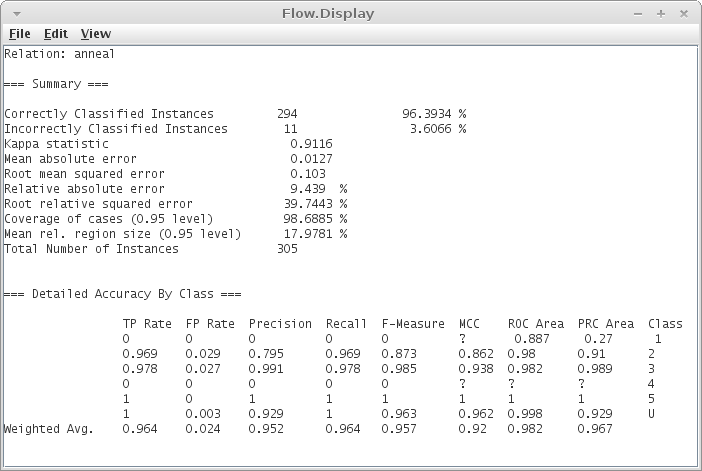
\includegraphics[width=5.5cm]{images/basic-randomspliteval-output.png}
    \caption{Summary output of classifier built/evaluated on random split.}
    \label{basic-randomspliteval-output}
  \end{minipage}
\end{figure}

Figures \ref{basic-traintestseteval-flow} and
\ref{basic-traintestseteval-output} display the flow\footnote{adams-weka-assemble\_traintestset\_container\_and\_evaluate\_classifier.flow}
for manually creating a container using the general purpose
\textit{MakeContainer} source actor. In order to assemble a container, you need
to know \textbf{what} type of container you want to create (the type is normally
listed in the ``Help'' of an actor), \textbf{where} to obtain the data from
(i.e., the callable actors) and \textbf{how} to store the data (i.e., under which
name in the container).

\begin{figure}[ht]
  \begin{minipage}[t]{0.5\linewidth}
    \centering
    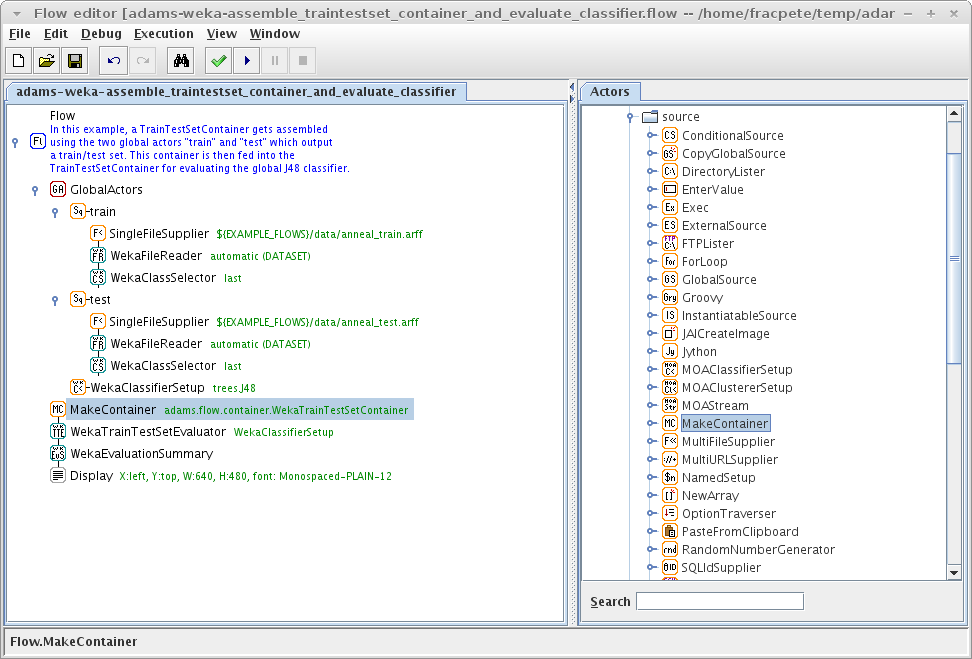
\includegraphics[width=6.0cm]{images/basic-traintestseteval-flow.png}
    \caption{Flow for evaluating classifier on separate train/test set.}
    \label{basic-traintestseteval-flow}
  \end{minipage}
  \hspace{0.5cm}
  \begin{minipage}[t]{0.5\linewidth}
    \centering
    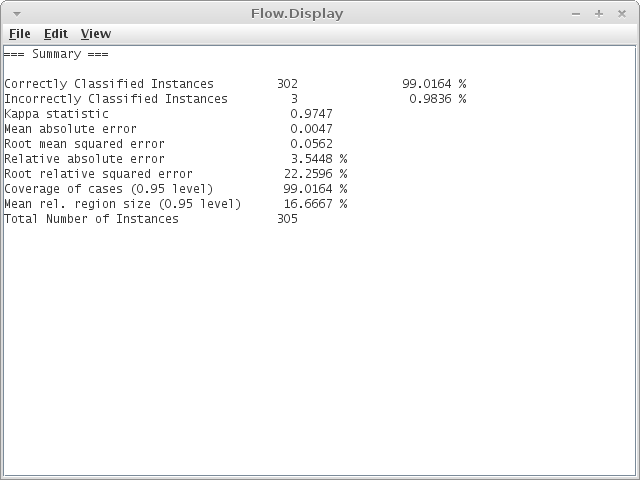
\includegraphics[width=5.5cm]{images/basic-traintestseteval-output.png}
    \caption{Summary output of classifier evaluated on separate train/test set.}
    \label{basic-traintestseteval-output}
  \end{minipage}
\end{figure}

\heading{Stream evaluation}
Though WEKA is usually used for batch-training, it is also possible to perform
incremental training and evaluation, as long as the classifier in use is an
\textit{updateable} one (i.e., it implements the \textit{weka.classifiers.Updateable}
interface). In such a scenario, you only have to read in the data incrementally
(changing the set up in the \textit{WekaFileReader} to \textit{INCREMENTAL})
and use the \textit{WekaStreamEvaluator} transformer for performing the
evaluation. The \textit{WekaStreamEvaluator} actor use prequential evaluation,
i.e., first evaluate, then train. Figure \ref{basic-streameval-flow} shows a 
flow that evaluates a \textit{NaiveBayesUpdateable} on a stream of data, 
displaying the textual evaluation summary and ROC (receiver operator curve) 
every 100 instances that come through.

\begin{figure}[ht]
  \begin{minipage}[t]{0.5\linewidth}
    \centering
    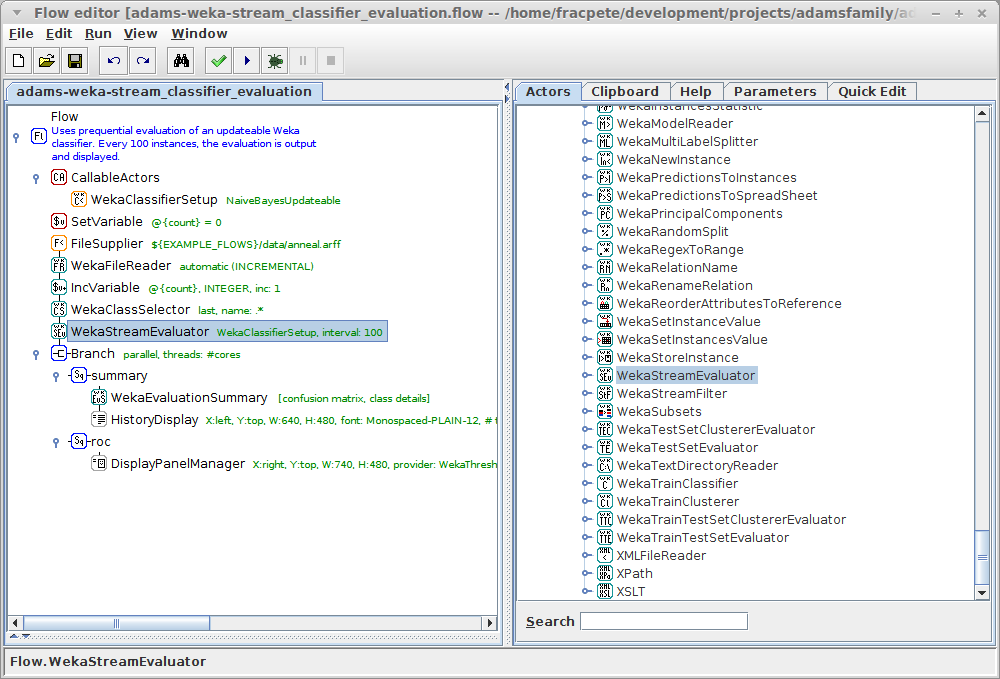
\includegraphics[width=12.0cm]{images/basic-streameval-flow.png}
    \caption{Flow for evaluating updateable classifier on data stream.}
    \label{basic-streameval-flow}
  \end{minipage}
\end{figure}

\begin{figure}[ht]
  \begin{minipage}[t]{0.5\linewidth}
    \centering
    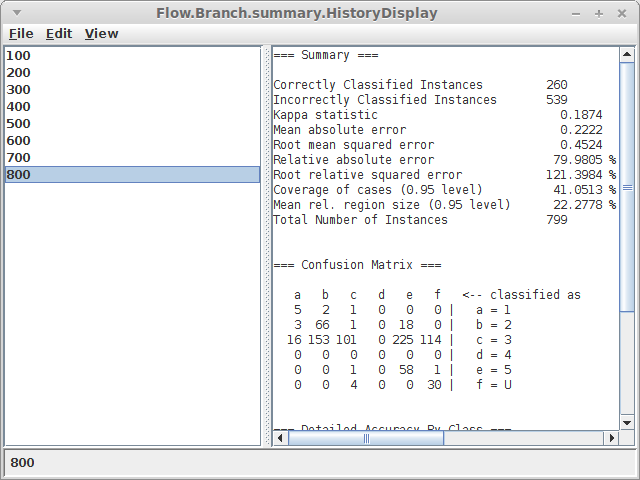
\includegraphics[width=5.5cm]{images/basic-streameval-output.png}
    \caption{Summary output of classifier evaluated on data stream.}
    \label{basic-streameval-output}
  \end{minipage}
  \hspace{0.5cm}
  \begin{minipage}[t]{0.5\linewidth}
    \centering
    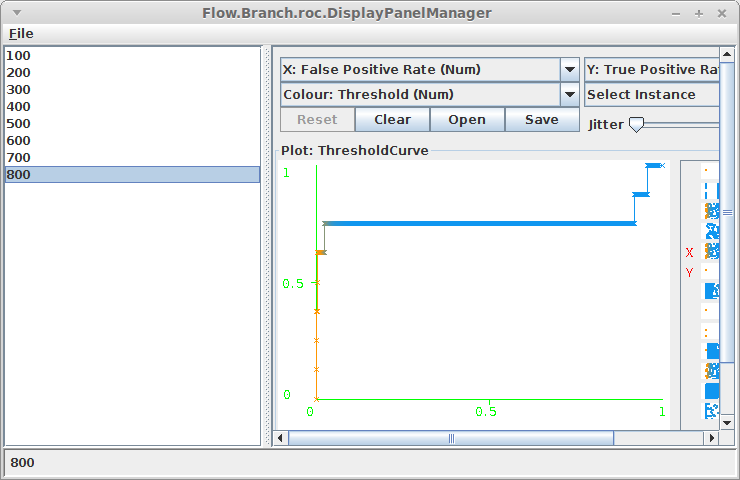
\includegraphics[width=5.5cm]{images/basic-streameval-output2.png}
    \caption{ROC curves of classifier evaluated on data stream.}
    \label{basic-streameval-output2}
  \end{minipage}
\end{figure}


\heading{Visualization}
You have already encountered the display of the classifier errors (in Figure
\ref{basic-preprocessing_errors-original}). The sink for displaying these errors
is \textit{WekaClassifierErrors}, which takes an \textit{Evaluation} object as
input. If you want to evaluate and display multiple classifiers then you have to
use the \textit{DisplayPanelManager} with the \textit{WekaClassifierErrors}
actor as ``panelProvider''. The \textit{DisplayPanelManager} actor offers a
history of generated panels, like the \textit{HistoryDisplay} does for plain
text.

Another interesting visualization is the \textit{WekaAccumulatedError}
transformer. This transformer takes also an \textit{Evaluation} object and then
turns it into a special sequence of plot containers: it creates a sequence of
the prediction errors that were obtained during an evaluation and outputs them
sorted, from smallest to
largest\footnote{adams-weka-accumulated\_error\_display.flow}. The Figures
\ref{basic-accumulatederror-flow} and \ref{basic-accumulatederror-output} show
the flow and the generated output respectively. As you can see from the graph,
GaussianProcesses generates consistently larger errors than LinearRegression,
which only seems to have a few big outliers (steep increase at the end).

\begin{figure}[ht]
  \begin{minipage}[t]{0.5\linewidth}
    \centering
    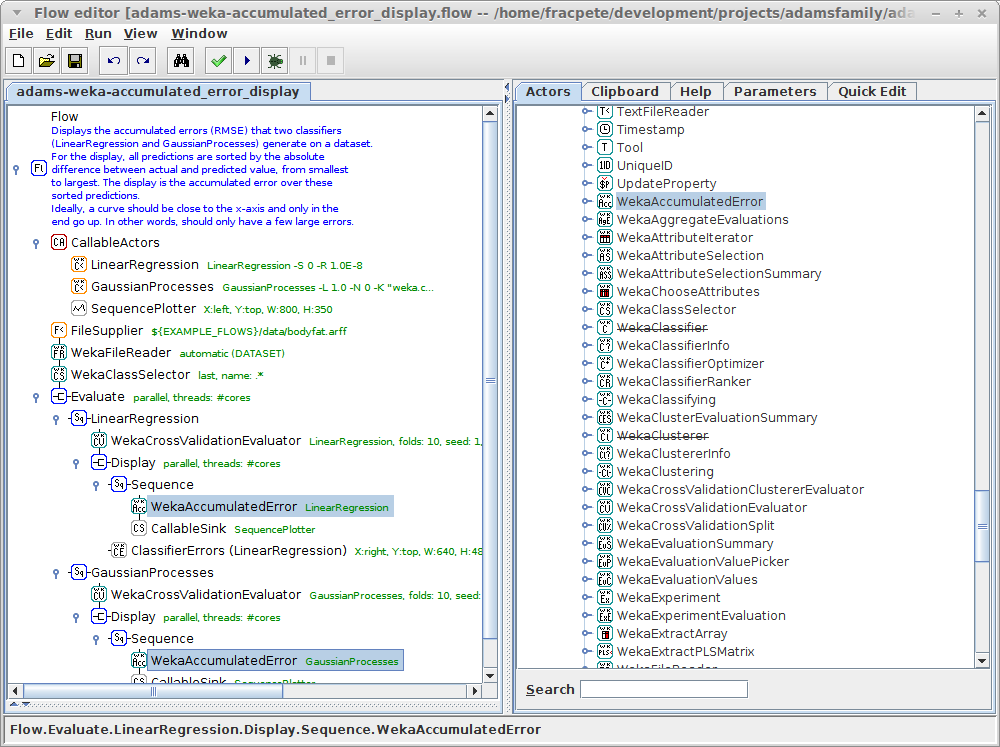
\includegraphics[width=6.0cm]{images/basic-accumulatederror-flow.png}
    \caption{Flow for displaying the ``accumulated error'' of a two
    classifiers.}
    \label{basic-accumulatederror-flow}
  \end{minipage}
  \hspace{0.5cm}
  \begin{minipage}[t]{0.5\linewidth}
    \centering
    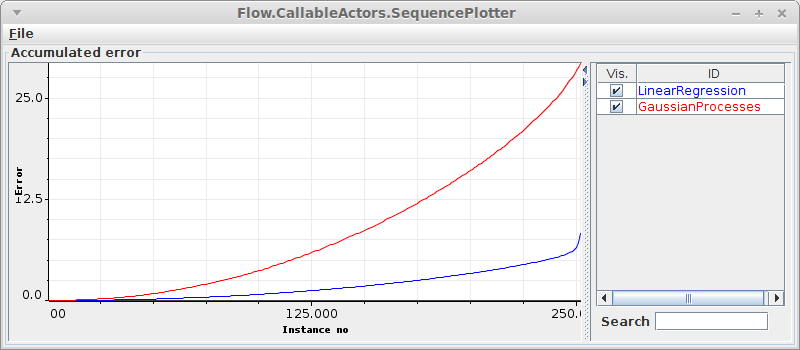
\includegraphics[width=5.5cm]{images/basic-accumulatederror-output.png}
    \caption{The ``accumulated error'' of LinearRegression and
    GaussianProcesses.}
    \label{basic-accumulatederror-output}
  \end{minipage}
\end{figure}

\clearpage
\subsection{Making predictions}
Of course, building models is only part of the picture. You will want to use
this model as well and make predictions with it. The actor for making
predictions on incoming data (i.e., single instance objects) is the
\textit{WekaClassifying} actor. This actor can either use a serialized model or
a callable actor that generates a trained classifier. The
flow\footnote{adams-weka-classifying\_data.flow} in Figure
\ref{basic-classifying-flow} uses the callable actor approach, training a
classifier on a training set and then performing classifications on a test set,
with the class distributions shown on screen (see Figure
\ref{basic-classifying-output}).

\begin{figure}[ht]
  \begin{minipage}[t]{0.5\linewidth}
    \centering
    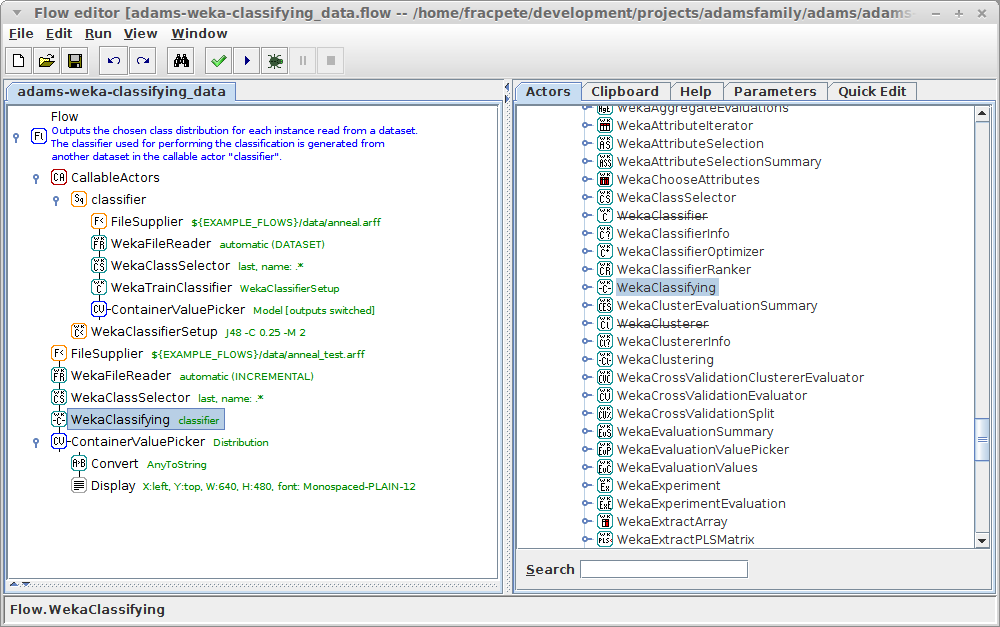
\includegraphics[width=6.0cm]{images/basic-classifying-flow.png}
    \caption{Flow for classifying new data and outputting the class
    distributions.}
    \label{basic-classifying-flow}
  \end{minipage}
  \hspace{0.5cm}
  \begin{minipage}[t]{0.5\linewidth}
    \centering
    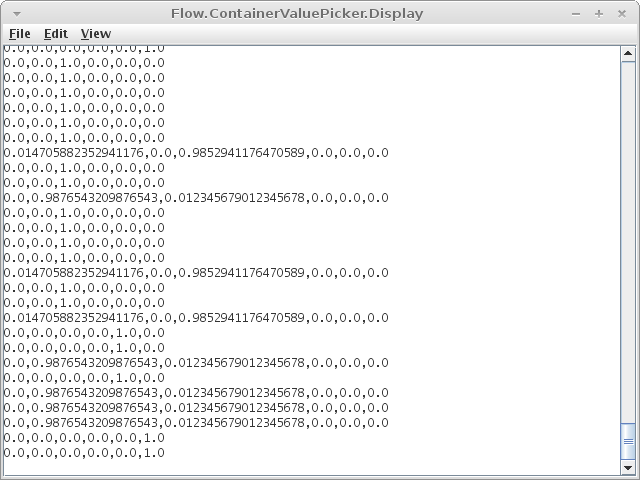
\includegraphics[width=5.5cm]{images/basic-classifying-output.png}
    \caption{The generated class distributions for the new data.}
    \label{basic-classifying-output}
  \end{minipage}
\end{figure}

\newpage
\section{Advanced}

\subsection{Learning curves}
Classifiers are susceptible to the order and amount of data that they are
trained with. Using learning curves, one can investigate how the data
influences the classifier performance.

Figures \ref{advanced-learning_curve-incremental-flow} and \ref{advanced-learning_curve-incremental-output}
show a flow and the generated output of an incremental NaiveBayes classifier, 
with the classifier being evaluated against a test set every 10 training 
instances (\textit{ConditionalTee} in conjunction with the \textit{Counting}
condition).\footnote{adams-weka-build\_classifier\_incrementally.flow}

\begin{figure}[ht]
  \begin{minipage}[t]{0.55\linewidth}
    \centering
    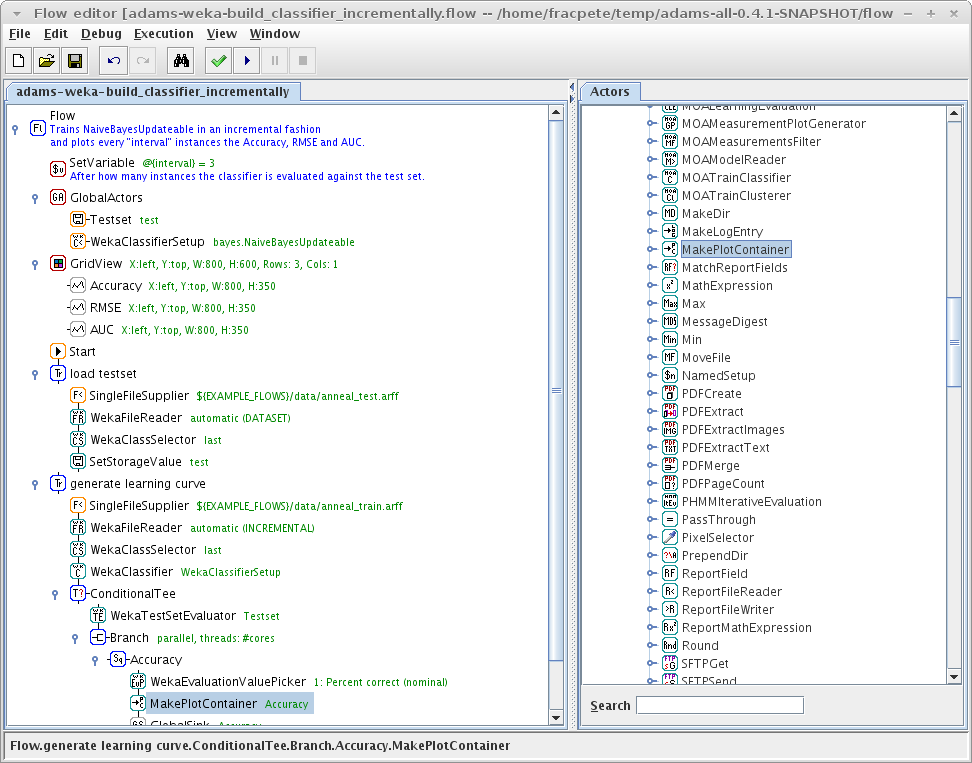
\includegraphics[width=7.0cm]{images/advanced-learning_curve-incremental-flow.png}
    \caption{Flow for generating learning curve for incremental classifier.}
    \label{advanced-learning_curve-incremental-flow}
  \end{minipage}
  \hspace{0.5cm}
  \begin{minipage}[t]{0.45\linewidth}
    \centering
    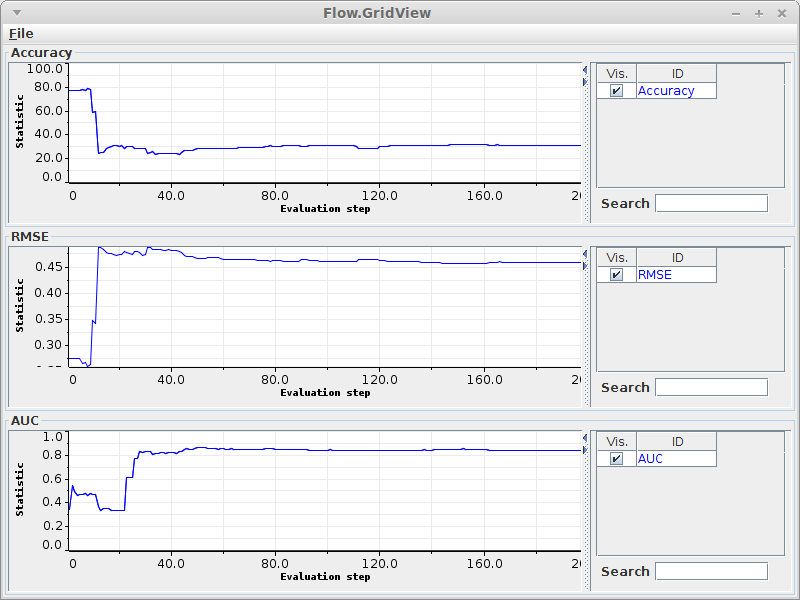
\includegraphics[width=4.5cm]{images/advanced-learning_curve-incremental-output.png}
    \caption{Generated learning curve (incremental).}
    \label{advanced-learning_curve-incremental-output}
  \end{minipage}
\end{figure}

Incremental classifiers are great for generating these kind of graphs. But
even for batch classifiers you can generate learning curves. Using the 
\textit{WekaInstanceBuffer} transformer, it is possible to buffer instances as
they come through and output datasets with which the batch classifer can get
trained (and evaluated). Figures \ref{advanced-learning_curve-batch-flow} and
\ref{advanced-learning_curve-incremental-output} show how to generate a 
learning curve for the decision tree classifier J48, being evaluated every
10 instances.\footnote{adams-weka-classifier\_learning\_curve.flow}

\begin{figure}[ht]
  \begin{minipage}[t]{0.55\linewidth}
    \centering
    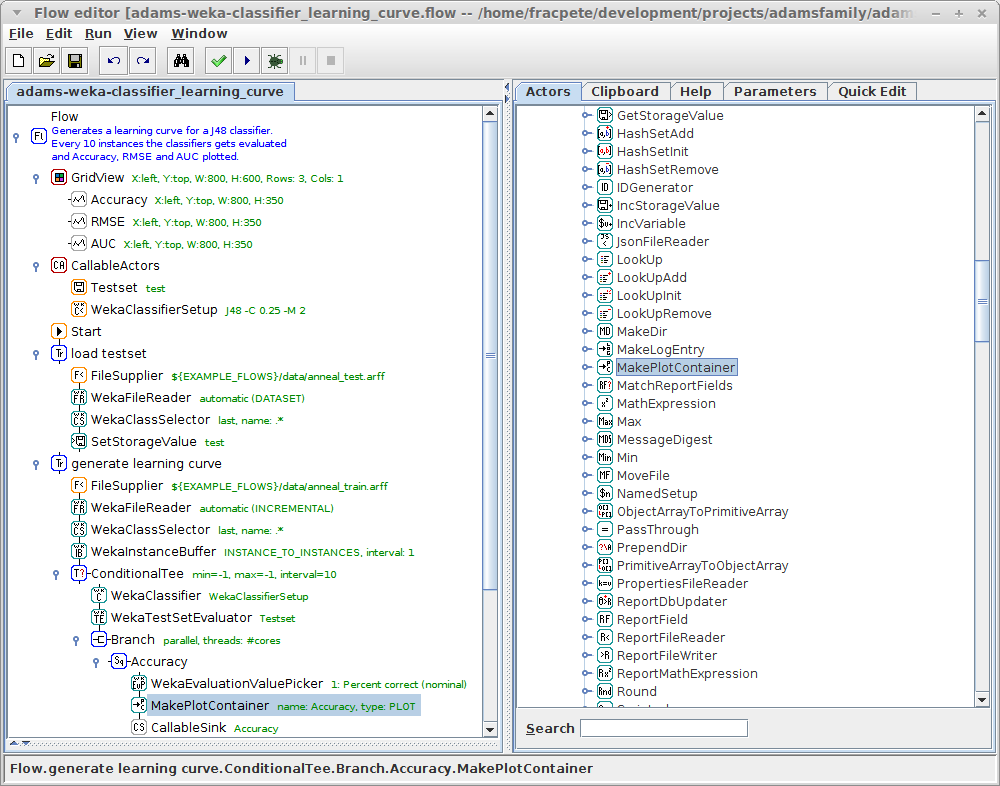
\includegraphics[width=7.0cm]{images/advanced-learning_curve-batch-flow.png}
    \caption{Flow for generating learning curve for batch classifier.}
    \label{advanced-learning_curve-batch-flow}
  \end{minipage}
  \hspace{0.5cm}
  \begin{minipage}[t]{0.45\linewidth}
    \centering
    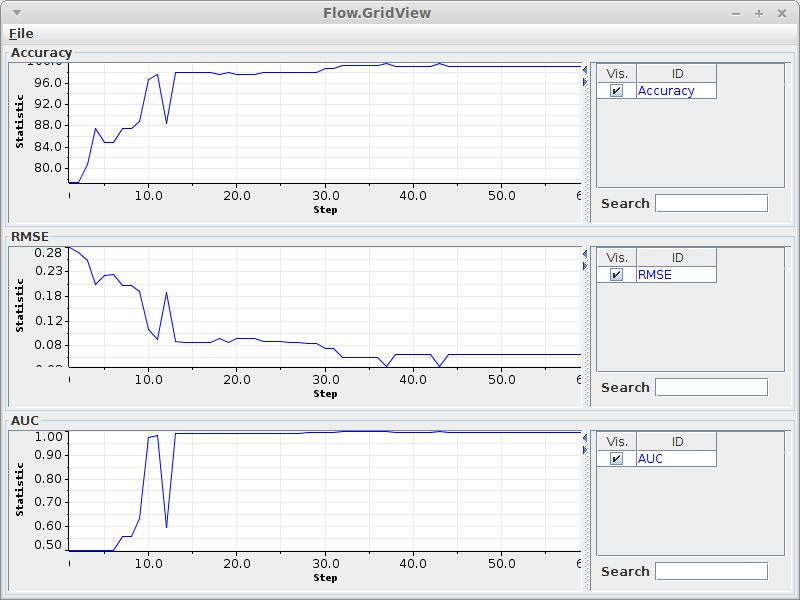
\includegraphics[width=4.5cm]{images/advanced-learning_curve-batch-output.png}
    \caption{Generated learning curve (batch).}
    \label{advanced-learning_curve-batch-output}
  \end{minipage}
\end{figure}

\subsection{Experiments}
For generating and execution experiments, you have two options: use the
existing Weka framework or the more flexible one provided by ADAMS (it
still uses the same Weka methods for generating the statistics).

For using the Weka framework, have a look at the following flows:
\begin{tight_itemize}
  \item experiment generation -- \textit{adams-weka-experiment\_generation.flow}
  \item execution and evaluation -- \textit{adams-weka-experiment.flow}
\end{tight_itemize}

For using the ADAMS framework, check out these:
\begin{tight_itemize}
  \item \textit{adams-weka-experiment2.flow}
  \item \textit{adams-weka-experiment3.flow}
\end{tight_itemize}

\subsection{Optimization}
The following flows demonstrate some of the optimization capabilities:
\begin{tight_itemize}
  \item setup generators -- \textit{adams-weka-classifier\_setup\_generation.flow},
  \item ranker -- \textit{adams-weka-classifier\_setup\_ranking.flow},
  \item optimizer -- \textit{adams-weka-classifier\_optimizer.flow}
\end{tight_itemize}

You can also use the \textit{WekaGeneticAlgorithm} transformer to optimize on an incoming
dataset.

\subsection{Partial Least Squares}
Using the \textit{WekaExtractPLSMatrix} transformer, you can extract various
PLS matrices from a \textit{PLSFilterWithLoadings} filter or a 
\textit{PLSClassifierWeightedWithLoadings} classifier (or a \textit{WekaModelContainer},
if this container should have a \textit{PLSClassifierWeightedWithLoadings} classifier 
stored).\footnote{adams-weka-extract\_pls\_matrix.flow}
You can also use the \textit{WekaGenericPLSMatrixAccess} transformer.

\subsection{Ensembles}
With the \textit{WekaEnsembleGenerator} it is possible to create ensembles from
input data (like pre-built classifiers) rather than training the ensemble itself.
With the \textit{VotedModels} generator, you can create a \textit{Vote}
meta-classifier from the incoming classifier array, using the supplied Vote
template.\footnote{adams-weka-lts-create\_vote\_ensemble.flow}



% Copyright (c) 2009-2012 by the University of Waikato, Hamilton, NZ. 
% This work is made available under the terms of the 
% Creative Commons Attribution-ShareAlike 3.0 license, 
% http://creativecommons.org/licenses/by-sa/3.0/. 
%
% Version: $Revision$

\chapter{Clustering}
\label{clustering}
Clustering behaves very much like Classification/Regression, the only difference
being that it is an unsupervised learning process. This means that the flows
won't contain a \textit{WekaClassSelector} actor to set the class attribute in
the loaded data. Due to the similarity, the section here will cover only
the basics of clustering.

\section{Building models}
Building clustering models is as easy as building classification/regression
models. Instead of the \textit{WekaTrainClassifier} transformer, you use the
\textit{WekaTrainClusterer} one. Similar, you use a \textit{WekaClustererSetup}
source instead of the \textit{WekaClassifierSetup} one to define (and output)
a clusterer setup, placed inside a \textit{CallableActors} standalone.

Figures \ref{build_clusterer-flow} and \ref{build_clusterer-output} show a flow
\footnote{adams-weka-build\_clusterer.flow} that builds a \textit{SimpleKMeans}
clusterer on a dataset (the class attribute gets removed using a
\textit{WekaFilter} actor) and the generated model gets displayed.

\begin{figure}[ht]
  \begin{minipage}[t]{0.5\linewidth}
    \centering
    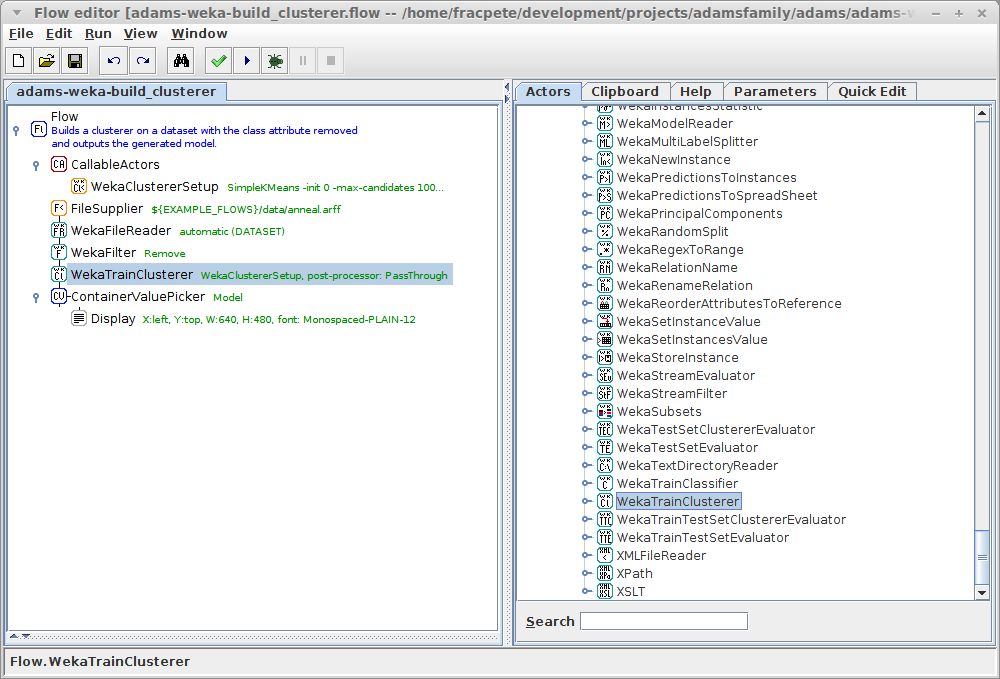
\includegraphics[width=6.0cm]{images/build_clusterer-flow.png}
    \caption{Building a clusterer and outputting the model.}
    \label{build_clusterer-flow}
  \end{minipage}
  \hspace{0.5cm}
  \begin{minipage}[t]{0.5\linewidth}
    \centering
    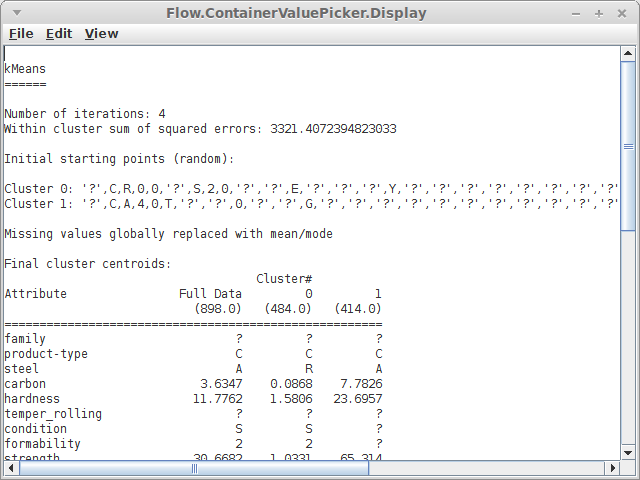
\includegraphics[width=5.5cm]{images/build_clusterer-output.png}
    \caption{Cluster model output.}
    \label{build_clusterer-output}
  \end{minipage}
\end{figure}

If the base cluster algorithm is an incremental one, i.e., one that implements
the \textit{weka.clusterers.UpdateableClusterer} interface, you can build your
clustering model incrementally as well. The flow
\footnote{adams-weka-build\_clusterer\_incrementally.flow} in Figure
\ref{build_clusterer_incrementally-flow} builds the CobWeb cluster algorithm
incrementally and outputs the generated models every 25 instances (see Figure
\ref{build_clusterer_incrementally-output}).

\begin{figure}[ht]
  \begin{minipage}[t]{0.5\linewidth}
    \centering
    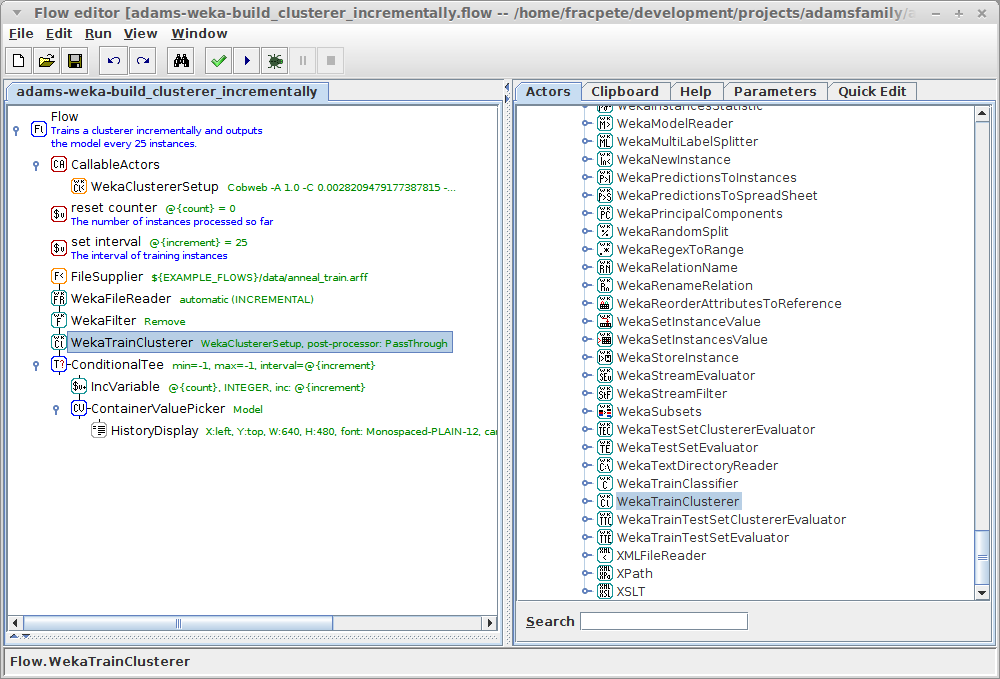
\includegraphics[width=6.0cm]{images/build_clusterer_incrementally-flow.png}
    \caption{Building a clusterer incrementally and outputting the model.}
    \label{build_clusterer_incrementally-flow}
  \end{minipage}
  \hspace{0.5cm}
  \begin{minipage}[t]{0.5\linewidth}
    \centering
    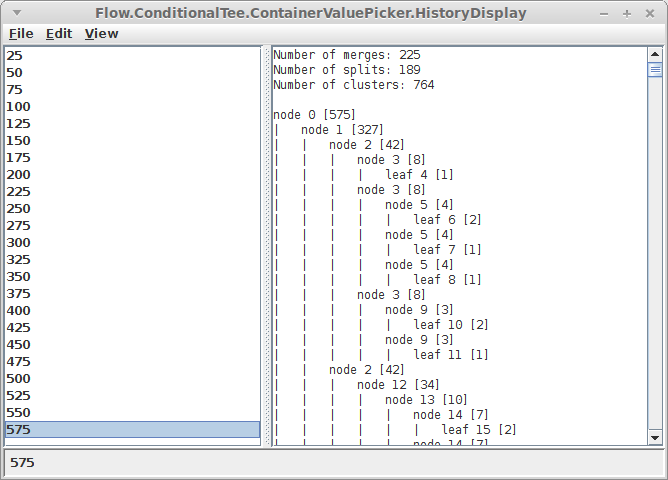
\includegraphics[width=5.5cm]{images/build_clusterer_incrementally-output.png}
    \caption{Cluster model outputs, generated every 25 instances.}
    \label{build_clusterer_incrementally-output}
  \end{minipage}
\end{figure}

\section{Evaluating clusterers}
ADAMS offers transformers for evaluation clusterers on data similar to the 
ones for classification:
\begin{tight_itemize}
	\item \textit{WekaClusterEvaluationSummary} - generates a string representation
	of a cluster evaluation (or container)
	\item \textit{WekaCrossValidationClustererEvaluator} - cross-validates a
	clusterer on a dataset, generates log-likelhood.
	\item \textit{WekaTestSetClustererEvaluator} - evaluates a built clusterer
	on a test set.
	\item \textit{WekaTrainTestSetClustererEvaluator} - builds and evaluates
	a clusterer on the training and test set from a train/test-set container.
\end{tight_itemize}

\section{Clustering data}
Clustering new data is done using the \textit{WekaClustering} transformer, which
takes a single instance as input and outputs the generated clustering
information in form of a container (\textit{WekaClusteringContainer}). You can
either specify a serialized clusterer model to use or a global actor to obtain
the clusterer from. The flow \footnote{adams-weka-clustering\_data.flow} in
Figure \ref{clustering-flow} shows how to build a clusterer and use it to
cluster new data, outputting the cluster distributions (see Figure
\ref{clustering-output} for the generated output).

\begin{figure}[ht]
  \begin{minipage}[t]{0.5\linewidth}
    \centering
    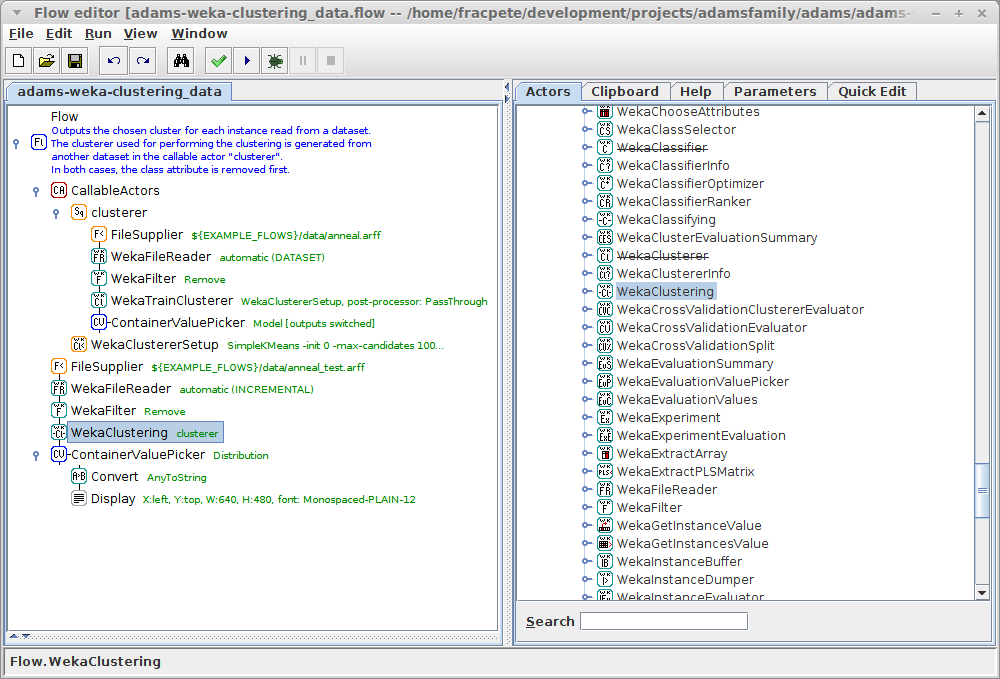
\includegraphics[width=6.0cm]{images/clustering-flow.png}
    \caption{Flow for clustering new data.}
    \label{clustering-flow}
  \end{minipage}
  \hspace{0.5cm}
  \begin{minipage}[t]{0.5\linewidth}
    \centering
    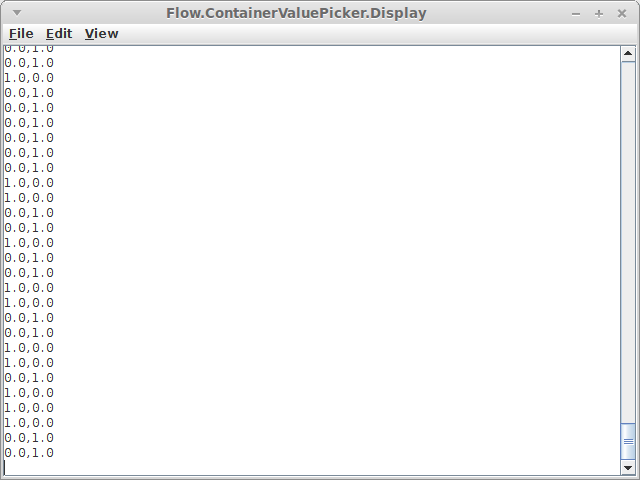
\includegraphics[width=5.5cm]{images/clustering-output.png}
    \caption{Generated cluster.}
    \label{clustering-output}
  \end{minipage}
\end{figure}


% This work is made available under the terms of the
% Creative Commons Attribution-ShareAlike 3.0 license, 
% http://creativecommons.org/licenses/by-sa/3.0/. 
%
% Version: $Revision$

\chapter{Attribute selection}
\label{attribute_selection}
ADAMS also offers WEKA's functionality for attribute selection and ranking.
The following transformers are available:
\begin{tight_itemize}
	\item \textit{WekaAttributeSelection} -- performs the attribute 
	selection/ranking.
	\item \textit{WekaAttributeSelectionSummary} -- generates a summary from
	a attribute selection step.
\end{tight_itemize}

In Figure \ref{attribute-selection_flow} you can see a flow\footnote{adams-weka-attribute\_selection-subset.flow} 
that uses \textit{CfsSubsetEval} as the attribute set evaluator and \textit{BestFirst}
as the search method. The generated output, summary and reduced dataset,
are displayed in Figures \ref{attribute-selection_output1} and 
\ref{attribute-selection_output2}.

\begin{figure}[htb]
  \centering
  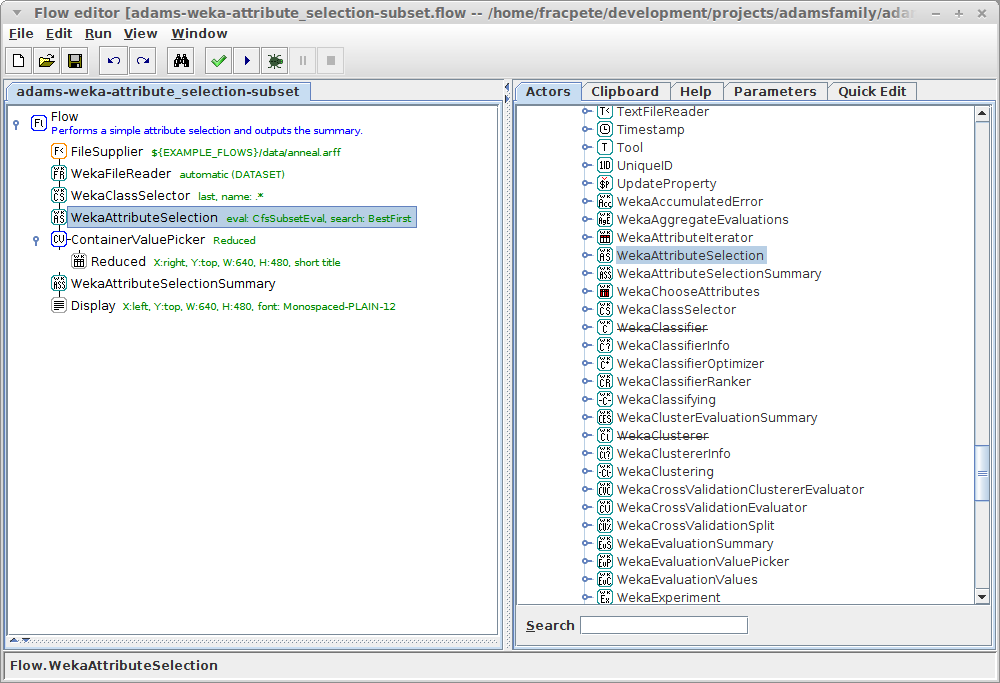
\includegraphics[width=6.0cm]{images/attribute-selection_flow.png}
  \caption{Flow for performing attribute selection (reduction).}
  \label{attribute-selection_flow}
\end{figure}

\begin{figure}[ht]
  \begin{minipage}[t]{0.5\linewidth}
    \centering
    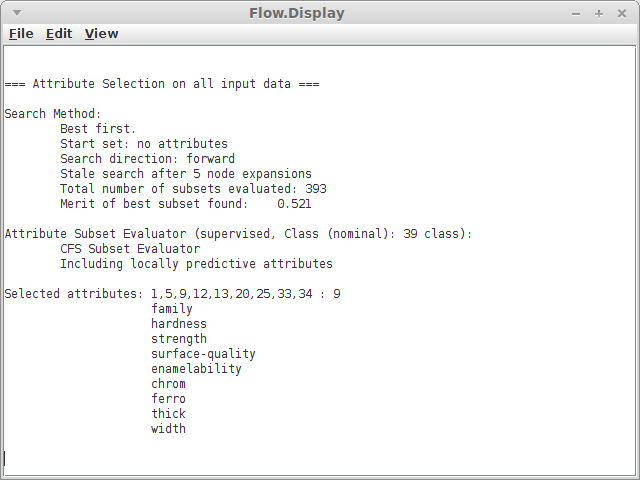
\includegraphics[width=6.0cm]{images/attribute-selection_output1.png}
    \caption{Summary of the reduction.}
    \label{attribute-selection_output1}
  \end{minipage}
  \hspace{0.5cm}
  \begin{minipage}[t]{0.5\linewidth}
    \centering
    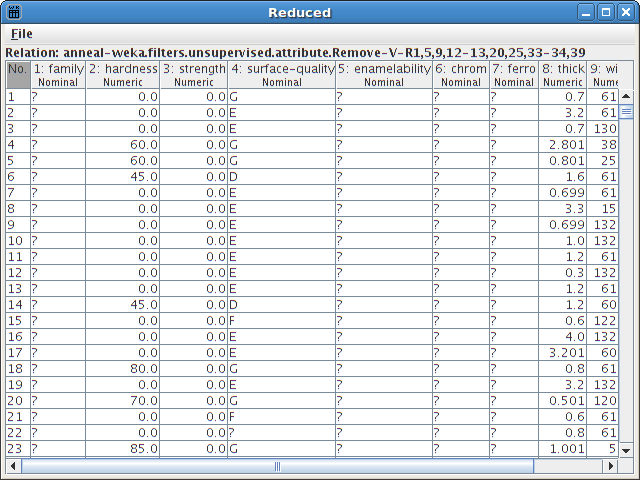
\includegraphics[width=5.5cm]{images/attribute-selection_output2.png}
    \caption{The reduced dataset.}
    \label{attribute-selection_output2}
  \end{minipage}
\end{figure}

The \textit{WekaAttributeSelection} transformer outputs a container which can 
contain the following elements:
\begin{tight_itemize}
	\item \textit{Train} -- the training set.
	\item \textit{Reduced} -- the reduced dataset.
	\item \textit{Transformed} -- the transformed dataset, in case of evaluators that 
	implement \textit{AttributeTransformer}, like principal components.
	\item \textit{Evaluation} -- the generated attribute selection evaluation.
	\item \textit{Statistics} -- a spreadsheet with statistics, containing
	information whether an attribute was selected (0 or 1) or for ranking results
	the rank of the attribute.
	\item \textit{Seed} -- the seed value in case of cross-validation.
	\item \textit{Folds} -- the number of folds used in case of cross-validation.
\end{tight_itemize}


% Copyright (c) 2012 by the University of Waikato, Hamilton, NZ. 
% This work is made available under the terms of the 
% Creative Commons Attribution-ShareAlike 3.0 license, 
% http://creativecommons.org/licenses/by-sa/3.0/. 
%
% Version: $Revision$

\chapter{Visualization}

\section{Preview browser}
The WEKA module comes with custom viewers for serialized files. Apart from the
default view (Figure \ref{previewbrowser-default}), you can also view the
trees (Figure \ref{previewbrowser-tree}) and graphs (Figure \ref{previewbrowser-graph})
that some classifiers generate.

\begin{figure}[htb]
  \centering
  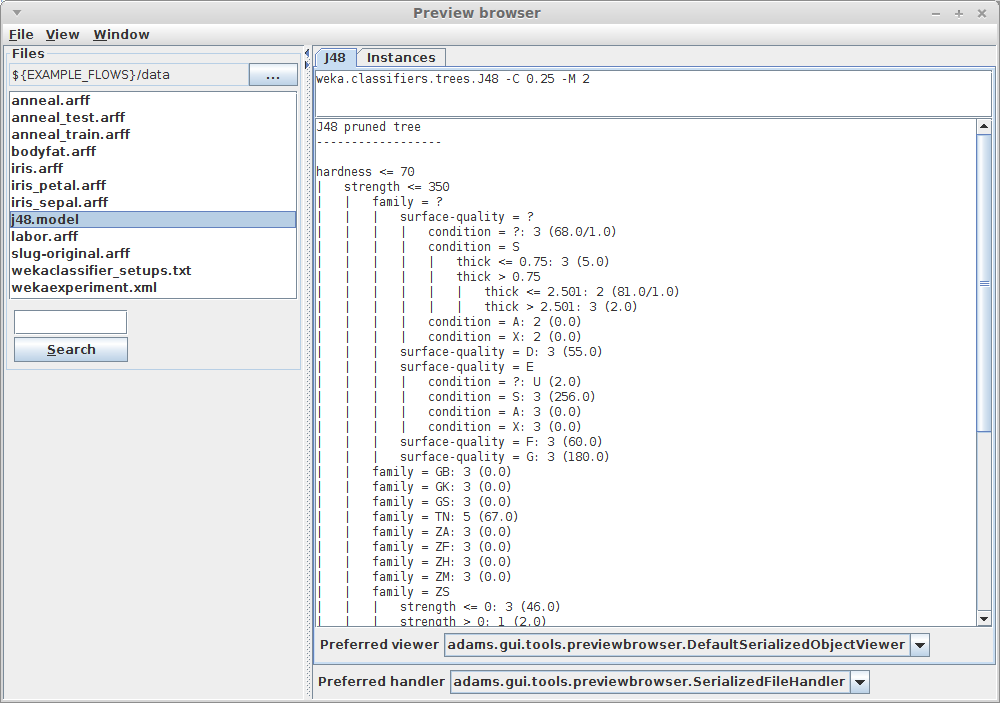
\includegraphics[width=10.0cm]{images/previewbrowser-default.png}
  \caption{Default preview for classifier.}
  \label{previewbrowser-default}
\end{figure}

\begin{figure}[htb]
  \centering
  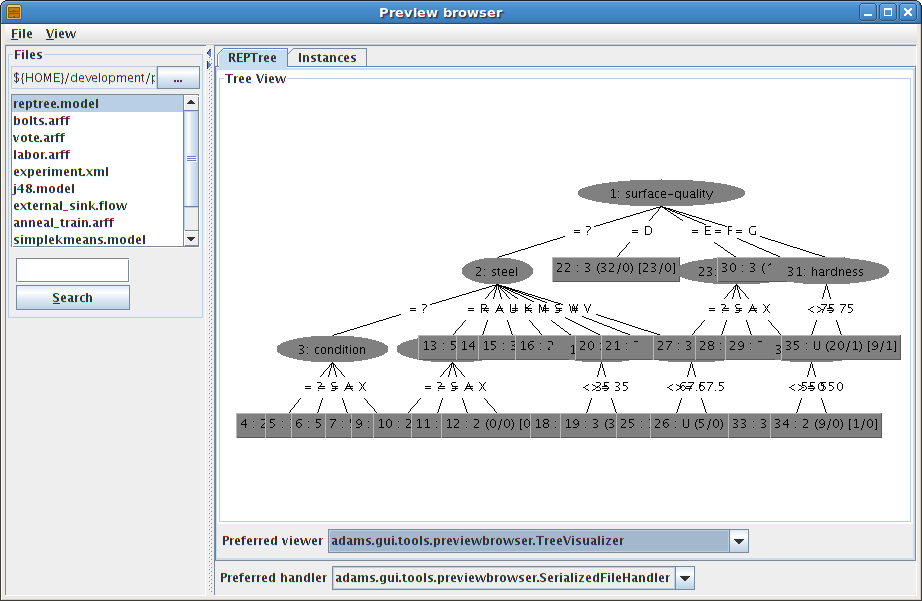
\includegraphics[width=10.0cm]{images/previewbrowser-tree.png}
  \caption{Preview of tree-generating classifier.}
  \label{previewbrowser-tree}
\end{figure}

\begin{figure}[htb]
  \centering
  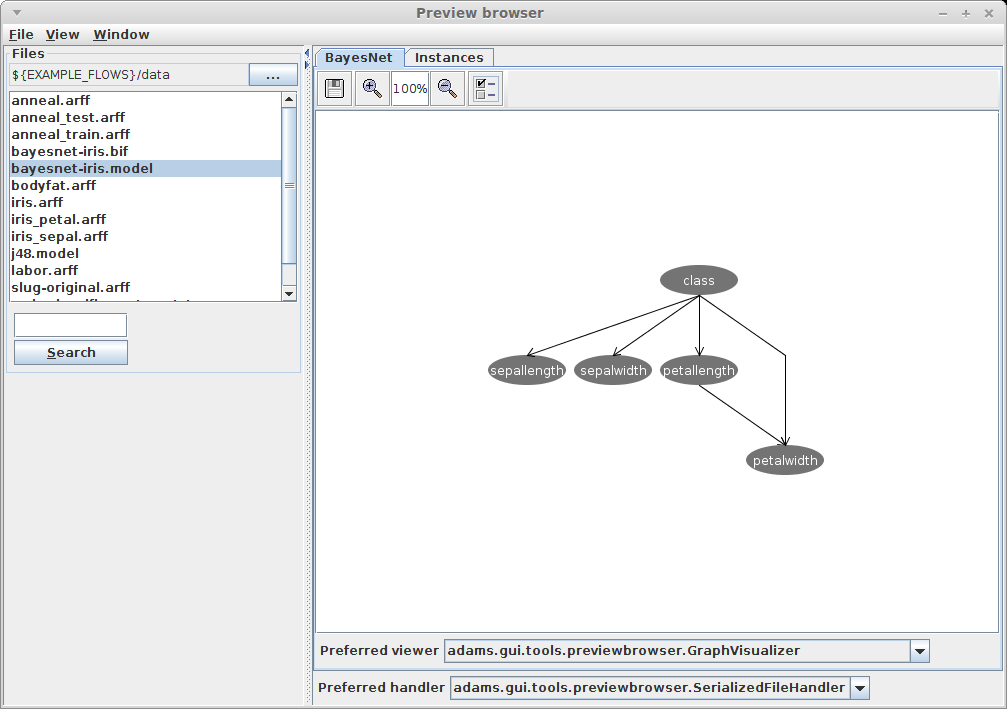
\includegraphics[width=10.0cm]{images/previewbrowser-graph.png}
  \caption{Preview for graph generated by BayesNet classifier.}
  \label{previewbrowser-graph}
\end{figure}


\clearpage
\section{Instance Compare}
Quite often, you generate data with different or tweaked pre-processing 
techniques and you wonder how different the generated data looks like.
The \textit{Instance Compare} visualization allows you to graphically compare
two datasets. You can either compare them row by row, or using a common 
attribute that can be used as unique row identifier.

Figure \ref{instance-compare} shows a comparison of two datasets. Not only
are the two rows overlayed, you also see the absolute difference plotter and
a the correlation coefficient of the two being calculated.

If you don't want to compare all the attributes, you can restrict it to a 
subset, by using the \textit{Att. range} text field. ``first'', ``second'',
``third'', ``last'', ``last\_1'' (last minus 1) and ``last\_2'' (last minus 2)
are accepted indices. All other indices must be 1-based.

\begin{figure}[htb]
  \centering
  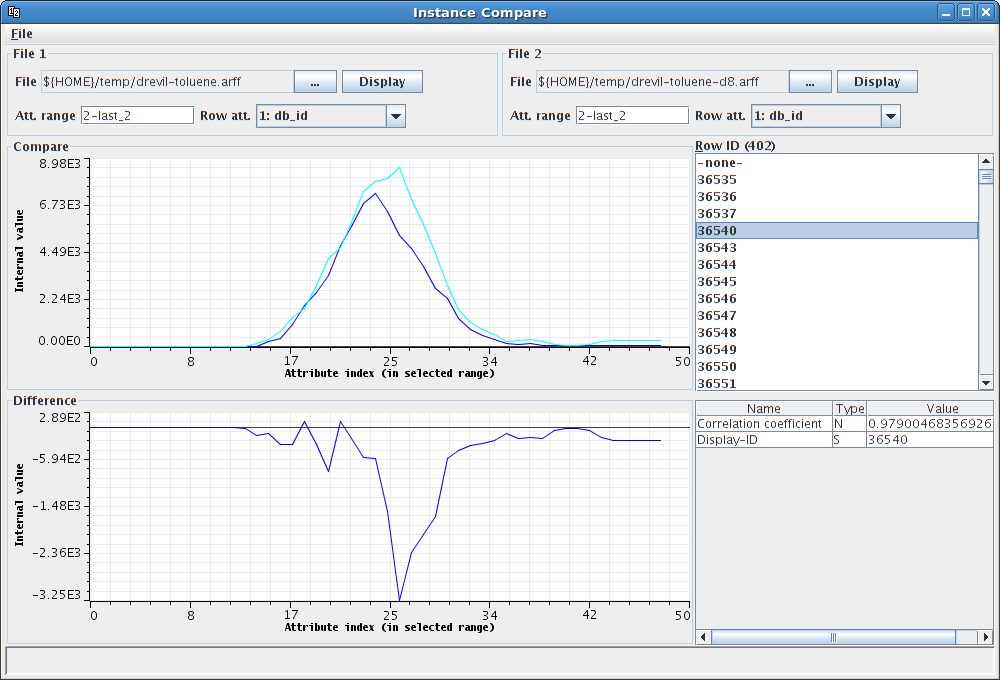
\includegraphics[width=10.0cm]{images/instance-compare.png}
  \caption{Comparing two datasets.}
  \label{instance-compare}
\end{figure}


\clearpage
\section{Instance Explorer}
When generating datasets, it pays to check the generated output in multiple
ways. For instance, whether the data rows generated are actually aligning 
properly. The \textit{Instance Explorer} allows you to select a range of
rows and columns from a dataset (see Figures \ref{instance-explorer_load1}
and \ref{instance-explorer_load2}), which are then displayed in a single
graph.

Figure \ref{instance-explorer_view} shows a subset of the UCI dataset
\textit{waveform-5000}. The top graph of the two is a zoom into the full graph, 
with the bottom graph showing the area that was zoomed into.

\begin{figure}[htb]
  \centering
  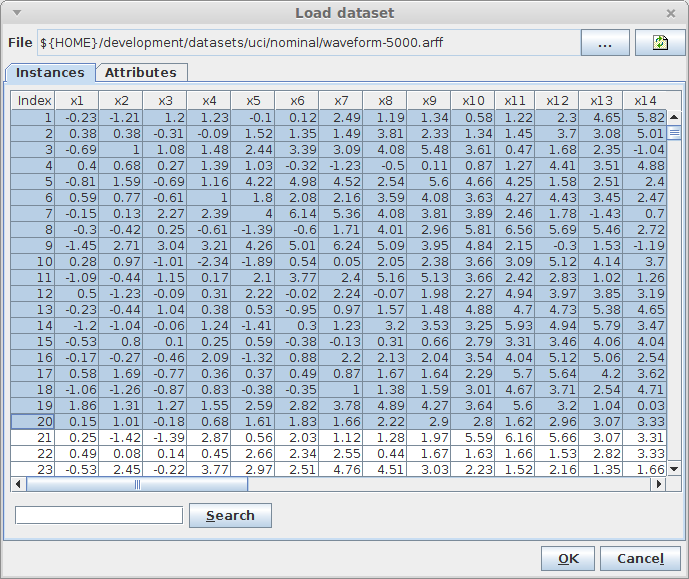
\includegraphics[width=10.0cm]{images/instance-explorer_load1.png}
  \caption{Viewing data in the Instance explorer.}
  \label{instance-explorer_load1}
\end{figure}

\begin{figure}[htb]
  \centering
  \includegraphics[width=10.0cm]{images/instance-explorer_load2.png}
  \caption{Viewing data in the Instance explorer.}
  \label{instance-explorer_load2}
\end{figure}

\begin{figure}[htb]
  \centering
  \includegraphics[width=10.0cm]{images/instance-explorer_view.png}
  \caption{Viewing data in the Instance explorer.}
  \label{instance-explorer_view}
\end{figure}


% Copyright (c) 2012-2013 by the University of Waikato, Hamilton, NZ. 
% This work is made available under the terms of the 
% Creative Commons Attribution-ShareAlike 3.0 license, 
% http://creativecommons.org/licenses/by-sa/3.0/. 
%
% Version: $Revision$

\chapter{Tools}

\section{Append datasets}

If you have datasets with the same structure, i.e., exactly the same
attributes, then you can use the \textit{Append datasets} tool to combine
them into a single, large dataset.

The screenshot in Figure \ref{dataset-compatibility} shows the wizard
interface that guides you through the process.

\begin{figure}[htb]
  \centering
  \includegraphics[width=12.0cm]{images/append_datasets.png}
  \caption{Appending datasets wizard.}
  \label{append_datasets}
\end{figure}

\clearpage
\section{Arff viewer}

WEKA's \textit{Arff viewer} is available from the ADAMS menu as well.

\begin{figure}[htb]
  \centering
  \includegraphics[width=12.0cm]{images/arffviewer.png}
  \caption{WEKA's Arff viewer displaying the iris UCI dataset.}
  \label{arffviewer}
\end{figure}

\clearpage
\section{Batch-filter datasets}

Training and test set are required to have exactly the same structure
in WEKA. If you need to apply a pre-processing filter to both of the
files, it is recommended to use \textit{batch-filtering}. This will
ensure that any statistics that get calculated based on the first
dataset, get applied to second file as well. An example for this is
the dictionary of the \textit{StringToWordVector}: the same word
dictionary needs to be applied to the second file, in order to generate
the same attributes. However, one usually has to resort to the command-line
in order to achieve this, which is rather tedious.

The \textit{Batch-filter datasets} wizard allows you to perform the
batch-filtering conveniently through the GUI:
\begin{tight_itemize}
  \item Select the datasets to filter (see \ref{batchfilter_datasets1})
  \item Configure the filter (see \ref{batchfilter_datasets2})
  \item Select the output directory (see \ref{batchfilter_datasets3})
  \item Info dialog after filtering (see \ref{batchfilter_datasets4})
\end{tight_itemize}

\begin{figure}[htb]
  \centering
  \includegraphics[width=12.0cm]{images/batchfilter_datasets1.png}
  \caption{Selecting input files for batch-filtering.}
  \label{batchfilter_datasets1}
\end{figure}

\begin{figure}[htb]
  \centering
  \includegraphics[width=12.0cm]{images/batchfilter_datasets2.png}
  \caption{Configuring the filter.}
  \label{batchfilter_datasets2}
\end{figure}

\begin{figure}[htb]
  \centering
  \includegraphics[width=12.0cm]{images/batchfilter_datasets3.png}
  \caption{Selecting the output directory for the filtered datasets.}
  \label{batchfilter_datasets3}
\end{figure}

\begin{figure}[htb]
  \centering
  \includegraphics[width=12.0cm]{images/batchfilter_datasets4.png}
  \caption{The dialog when batch-filtering was successful.}
  \label{batchfilter_datasets4}
\end{figure}

\clearpage
\section{BayesNet Editor}
WEKA's \textit{BayesNet Editor} allows you to view and modify Bayesian nets.
Figure \ref{bayesnet_editor} shows an example net loaded.

\begin{figure}[htb]
  \centering
  \includegraphics[width=12.0cm]{images/bayesnet_editor.png}
  \caption{BayesNet editor displaying a net.}
  \label{bayesnet_editor}
\end{figure}

\clearpage
\section{Dark Lord}
The \textit{Dark Lord} wizard allows you to set up and monitor a genetic
algorithm that determines the best set of attributes, based on the classifier
and metric you choose to optimize on. The output directory that you define
(see Figure \ref{darklord_setup}), is used to store all the \textit{reduced/optimized}
datasets that improved the metric. The optimization can be paused, resumed or
stopped with the buttons at the bottom right of the view panel (see Figure
\ref{darklord_run}).

\begin{figure}[htb]
  \centering
  \includegraphics[width=12.0cm]{images/darklord_setup.png}
  \caption{Dark Lord setup.}
  \label{darklord_setup}
\end{figure}

\begin{figure}[htb]
  \centering
  \includegraphics[width=12.0cm]{images/darklord_run.png}
  \caption{Dark Lord run.}
  \label{darklord_run}
\end{figure}

\clearpage
\section{Dataset compatibility}

WEKA requires training and test sets to have the same structure, down to the
same name and order of nominal labels. Rather than relying on the error message
in the Explorer, you can use the \textit{Dataset compatibility} tool to 
quickly check whether two or more datasets are actually compatible.

The screenshot in Figure \ref{dataset-compatibility} shows the output when
comparing two datases, one being the original \textit{anneal} UCI dataset
and the other one a transformed version.

\begin{figure}[htb]
  \centering
  \includegraphics[width=12.0cm]{images/dataset-compatibility.png}
  \caption{Compatibility output for two datasets.}
  \label{dataset-compatibility}
\end{figure}

\clearpage
\section{Explorer}
ADAMS contains an extended version of the WEKA Explorer. The interface uses
menus instead of buttons to declutter the pre-process tab. Also, it keeps track
of the datasets that the user loads, to make re-loading recent files easier.
This saves a lot of time when working with the same files on a frequent basis.
Furthermore, the user can have an arbitrary number of Explorer sessions in the
same window, distinguished by names. Figure \ref{explorerext} shows the new
interface with the drop-down menu in action.

\begin{figure}[htb]
  \centering
  \includegraphics[width=12.0cm]{images/explorerext.png}
  \caption{Explorer interface with menus.}
  \label{explorerext}
\end{figure}

One very useful feature is the notion of \textit{workspaces} in this interface.
You can save the current setup (current dataset, classifiers, clusterers,
evaluation set up, results, etc.) to a file and restore all of it in one go
again. Unfortunately, not all data can be stored, such as the log, the undo
history and the built models or visualizations associated with a results.
See Figure \ref{explorerext-workspaces} for the button (highlighted in red)
that allows you to load/save workspaces.

\begin{figure}[htb]
  \centering
  \includegraphics[width=12.0cm]{images/explorerext-workspaces.png}
  \caption{Saving/restoring of workspaces.}
  \label{explorerext-workspaces}
\end{figure}

\clearpage
\section{Make compatible datasets}
When dealing with data across multiple spreadsheets, e.g., training, test
and validation set, then it can happen that these datasets are not compatible
in the strict Weka sense.

The \textit{Make compatible datasets} wizard allows you to turn spreadsheets
into compatible ARFF files:
\begin{tight_itemize}
  \item Select the datasets to make compatible (see \ref{makecompatible1})
  \item Configure how the datasets are being read (see \ref{merge_datasets2})
  \item Select the output directory for the compatible ARFF files (see \ref{merge_datasets3})
  \item Info dialog after processing the datasets (see \ref{merge_datasets4})
\end{tight_itemize}

\begin{figure}[htb]
  \centering
  \includegraphics[width=12.0cm]{images/makecompatible1.png}
  \caption{Selecting input files for making compatible datasets.}
  \label{makecompatible1}
\end{figure}

\begin{figure}[htb]
  \centering
  \includegraphics[width=12.0cm]{images/makecompatible2.png}
  \caption{Configuring the readers for the datasets.}
  \label{makecompatible2}
\end{figure}

\begin{figure}[htb]
  \centering
  \includegraphics[width=12.0cm]{images/makecompatible3.png}
  \caption{Selecting the output directory for the compatible ARFF files.}
  \label{makecompatible3}
\end{figure}

\begin{figure}[htb]
  \centering
  \includegraphics[width=8.0cm]{images/makecompatible4.png}
  \caption{The dialog when dataset generation was successful.}
  \label{makecompatible4}
\end{figure}

\clearpage
\section{Merge datasets}
The process of adding reference data to a dataset or performing
\textit{data fusion}\footnote{\url{https://en.wikipedia.org/wiki/Data_fusion}{}},
can be quite often a manual process, copy/pasting datasets in a spreadsheet
application.

The \textit{Merge datasets} wizard allows you to perform the
process of combining datasets side-by-side conveniently in the GUI:
\begin{tight_itemize}
  \item Select the datasets to merge (see \ref{merge_datasets1})
  \item Configure the merge (see \ref{merge_datasets2})
  \item Select the output file (see \ref{merge_datasets3})
  \item Info dialog after merging (see \ref{merge_datasets4})
\end{tight_itemize}
Figure \ref{merge_datasets-output} shows an example of a merged file.

\begin{figure}[htb]
  \centering
  \includegraphics[width=12.0cm]{images/merge_datasets1.png}
  \caption{Selecting input files for merging.}
  \label{merge_datasets1}
\end{figure}

\begin{figure}[htb]
  \centering
  \includegraphics[width=12.0cm]{images/merge_datasets2.png}
  \caption{Configuring the merge.}
  \label{merge_datasets2}
\end{figure}

\begin{figure}[htb]
  \centering
  \includegraphics[width=12.0cm]{images/merge_datasets3.png}
  \caption{Selecting the output directory for the filtered datasets.}
  \label{merge_datasets3}
\end{figure}

\begin{figure}[htb]
  \centering
  \includegraphics[width=12.0cm]{images/merge_datasets4.png}
  \caption{The dialog when merging was successful.}
  \label{merge_datasets4}
\end{figure}

\begin{figure}[htb]
  \centering
  \includegraphics[width=12.0cm]{images/merge_datasets-output.png}
  \caption{The merged dataset.}
  \label{merge_datasets-output}
\end{figure}


%%%%%%%%%%%%%%%%%%%%%%%%%%%%%%%%%%%
% Copyright (c) 2009-2012 by the University of Waikato, Hamilton, NZ. 
% This work is made available under the terms of the 
% Creative Commons Attribution-ShareAlike 4.0 license,
% http://creativecommons.org/licenses/by-sa/4.0/.
%
% Version: $Revision$

\begin{thebibliography}{999}
	% to make the bibliography appear in the TOC
	\addcontentsline{toc}{chapter}{Bibliography}

    % references
	\bibitem{adams}
		\textit{ADAMS} -- Advanced Data mining and Machine learning System \\
		\url{https://adams.cms.waikato.ac.nz/}{}

	\bibitem{esrigrid}
	 	\textit{Esri Grid} -- a raster GIS file format deveoped by Esri. \\
		\url{https://en.wikipedia.org/wiki/Esri\_grid}{}

	\bibitem{kml}
	 	\textit{Keyhole Markup Language} -- an XML notation for expressing
	 	geographic annotation and visualization within Internet-based,
	 	two-dimensional maps and three-dimensional Earth browsers. \\
		\url{http://en.wikipedia.org/wiki/Keyhole\_Markup\_Language}{}

	\bibitem{postgresql}
	 	\textit{PostgreSQL} -- a powerful, open source object-relational
	 	database system. \\
		\url{http://www.postgresql.org/}{}

	\bibitem{postgis}
		\textit{PostGIS} -- a spatial database extender for PostgreSQL
		object-relational database. It adds support for geographic
		objects allowing location queries to be run in SQL.  \\
		\url{http://postgis.net/}{}

	\bibitem{srid4269}
	 	\textit{SRID 4269} -- or NAD 83 (North American Datum). \\
		\url{http://spatialreference.org/ref/epsg/4269/}{}

	\bibitem{mysql}
		\textit{MySQL} -- an open-source relational database management
		system (RDBMS) \\
		\url{http://www.mysql.com/}{}

\end{thebibliography}


\end{document}
